% The FYP template is designed according to NTU SCSE FYP guidelines on https://www3.ntu.edu.sg/scse/fyp/UsefulInfo/Report%20Guide.pdf.

% Credit
% Original version by Vincent Ribli
% https://www.overleaf.com/latex/templates/ntu-scse-fyp-template/kwdtcbqmjctk

% Revised by Prof Loy Chen Change
% 23 Aug 2024 - Replace SCSE with CCDS

\documentclass[pdftex, 12pt, a4paper]{report}
\usepackage[british]{babel}
\usepackage{newtxtext, newtxmath}
\usepackage[top=3cm, bottom=3cm, left=3.5cm, right=3cm]{geometry}
\usepackage[hidelinks]{hyperref}
\usepackage[pdftex]{graphicx}
\usepackage{booktabs}
\usepackage{setspace}
\usepackage{titlesec}
\usepackage{tocloft}
\usepackage{parskip}
\usepackage{amsmath}
\usepackage{amsfonts}
\usepackage{xcolor}
\usepackage{float}
\usepackage{soul}
\usepackage{microtype}
\usepackage[toc]{appendix}
\usepackage[sorting=none, style=ieee, ,citestyle=numeric-comp]{biblatex}

% Unicode support for file structure diagrams
\DeclareFieldFormat{urldate}{Accessed: #1}
\DeclareUnicodeCharacter{2588}{\rule{1ex}{\ht\strutbox}}
\DeclareUnicodeCharacter{251C}{\rule[-\dp\strutbox]{.4pt}{\baselineskip}%
  \rule[.2\baselineskip]{1ex}{.4pt}}
\DeclareUnicodeCharacter{2500}{\rule[.2\baselineskip]{1ex}{.4pt}}
\DeclareUnicodeCharacter{2514}{\rule[.2\baselineskip]{.4pt}{.5\baselineskip}%
  \rule[.2\baselineskip]{1ex}{.4pt}}
\DeclareUnicodeCharacter{2502}{\rule[-\dp\strutbox]{.4pt}{\baselineskip}}

% For code monospcae
% \definecolor{light-gray}{gray}{0.95}
% \newcommand{\code}[1]{\colorbox{light-gray}{\texttt{#1}}}
% For code snippets
\usepackage{listings}
\renewcommand\lstlistingname{Code}
\renewcommand\lstlistlistingname{List of Code Snippets}

\definecolor{dkgreen}{rgb}{0,0.6,0}
\definecolor{gray}{rgb}{0.5,0.5,0.5}
\definecolor{mauve}{rgb}{0.58,0,0.82}
\lstset{frame=tb,
  language={Python},
  aboveskip=3mm,
  belowskip=3mm,
  showstringspaces=false,
  columns=flexible,
  basicstyle={\small\ttfamily},
  numbers=none,
  numberstyle=\tiny\color{gray},
  keywordstyle=\color{blue},
  commentstyle=\color{dkgreen},
  stringstyle=\color{mauve},
  breaklines=true,
  breakatwhitespace=true,
  tabsize=3
}

\lstdefinelanguage{Proto3}{
  morekeywords={
    syntax, import, option, package, message, enum, repeated, optional, required,
    service, rpc, returns, int32, int64, uint32, uint64, sint32, sint64, fixed32,
    fixed64, sfixed32, sfixed64, bool, string, bytes, float, double
  },
  sensitive=true,
  morecomment=[l]{//},
  morecomment=[s]{/*}{*/},
  morestring=[b]",
}

\lstdefinelanguage{Terraform}{
  morekeywords={
    resource, provider, variable, output, module, terraform, locals, data,
    backend, provisioner, connection, lifecycle, depends_on, count, for_each,
    dynamic, if, else, for, in, end, true, false, null
  },
  sensitive=true,
  morecomment=[l]{//},
  morecomment=[s]{/*}{*/},
  morestring=[b]",
  morestring=[b]',
  morestring=[s]{<<}{>>},
}

\lstdefinelanguage{Kubernetes}{
  morekeywords={
    apiVersion, kind, metadata, spec, containers, name, image, ports, resources,
    requests, limits, deployment, replicas, selector, matchLabels, template, labels,
    app, service, type, NodePort, ports, targetPort, selector, ingress, rules, host,
    paths, path, backend, serviceName, servicePort, annotations, cert-manager.io/cluster-issuer,
    tls, secretName, spec, tls, hosts, secretName, issuerRef, name, namespace, spec, rules,
    metrics, scaleTargetRef, minReplicas, maxReplicas, resource, target, averageUtilization,
    host, http, paths, path, pathType, backend, service, port, status, loadBalancer, subjects, roleRef, apiGroup
  },
  alsoletter={kubernetes.io/service-account.name, kubernetes.io/service-account-token},
  sensitive=true,
  morecomment=[l]{//},
  morecomment=[s]{/*}{*/},
  morestring=[b]",
  morestring=[b]',
  morestring=[s]{<<}{>>},
}

\addbibresource{99-bibliography.bib}
\setstretch{1.5}
\setlength{\cftfigindent}{0pt}
\setlength{\cfttabindent}{0pt}
\renewcommand{\cftdotsep}{1}

% change the following
\title{\uppercase{Enhancing Speech Recognition Scalability and Resilience through Decoupled Architecture
}}
\newcommand\fypcode{CCDS24-0015}
\author{Tey Li Zhang Edmund}
\date{2025}
\newcommand\degree{Bachelor of Computing in Computer Science}

\begin{document}
\makeatletter
\begin{titlepage}
\begin{center}


\includegraphics[width=\textwidth]{figures/ntu_logo.png}
\\[2cm]

\uppercase{\textbf{\large{Nanyang Technological University}}}
\\[3cm]

\uppercase{\textbf{\large{\@title}}}

\vfill
\@author
\\[3cm]

Project Supervisor: Prof Chng Eng Siong\\
Examiner: A/P Douglas Leslie Maskell
\\[2cm]
College of Computing and Data Science\\
Academic Year 2024/2025

\end{center}
\end{titlepage}
\makeatother

\makeatletter
\begin{titlepage}
\begin{center}

\uppercase{\textbf{\large{Nanyang Technological University}}}
\\[6cm]

\uppercase{\textbf{\fypcode \\[0.3cm]\@title}}

\vfill

Submitted in Partial Fulfilment of the Requirements\\
for the Degree of \degree\\
of the Nanyang Technological University
\\[0.8cm]
by
\\[0.8cm]

\@author
\\[2cm]

\end{center}

College of Computing and Data Science\\
\@date
\end{titlepage}
\makeatother


\setcounter{page}{1}
\pagenumbering{roman}

\chapter*{Abstract}
\addcontentsline{toc}{chapter}{Abstract}

Automatic Speech Recognition (ASR) systems is an integral part of emergency call centers and other real-time transcription applications. To enhance the scalability and availability of the ASR system, this project redesigned the existing architecture to a decoupled architecture. The new design leverages RabbitMQ for asynchronous messaging, enabling independent scaling of system components and improving fault tolerance. A dynamic scaling policy is implemented to adjust worker instances based on real-time workload demands, optimizing resource utilization and maintaining low-latency processing. Fault recovery mechanisms are introduced to minimize service disruptions and ensure continuous transcription tasks. The system is deployed on Kubernetes clusters hosted on AWS, streamlining system management and enhancing scalability. Terraform is used for infrastructure-as-code to improve deployment reproducibility and operational efficiency. The project significantly enhances the system's scalability, reliability, and fault tolerance, benefiting NTU Speech Lab's research initiatives and critical applications such as SCDF's emergency call centers.

\chapter*{Acknowledgments}
\addcontentsline{toc}{chapter}{Acknowledgments}

I would like to thank my supervisor, Professor Chng Eng Siong, for his guidance and support throughout this project. His insightful feedback and advice have been instrumental in my learning journey. I am especially grateful for the opportunity to attend an AWS workshop, which significantly enhanced my cloud computing skills. 

I would also like to express my deepest gratitude to my mentor, Vu Thi Ly, whose continuous support and encouragement have been invaluable. Her guidance during our weekly meetings played a crucial role in shaping the direction of this project and ensuring its successful completion. Her prompt responses to my queries and her dedication to mentorship have made this an enriching and fulfilling experience.

Additionally, I would like to extend my sincere appreciation to my past internships at GovTech and the Central Provident Fund Board for providing me with the opportunity to work on various cloud computing projects. The knowledge and hands-on experience I gained from these internships has been instrumental in successfully completing this project.

Finally, I am profoundly grateful to my family and friends for their unwavering support, encouragement, and belief in me. Their constant motivation has been a driving force throughout my academic journey.


\pagebreak
\tableofcontents

\pagebreak
\phantomsection
\addcontentsline{toc}{chapter}{List of Figures}
\listoffigures

\pagebreak
\phantomsection
\addcontentsline{toc}{chapter}{List of Code Snippets}
\lstlistoflistings

\cleardoublepage
\pagenumbering{arabic}

\chapter{Introduction} \label{chapter:introduction}
\section{Background}

Automatic Speech Recognition (ASR) systems, which convert human speech into text, have become integral to modern voice-driven technologies. While current commercial ASR solutions excel in single-language environments, they often struggle with multilingual scenarios, due to inter- and intra-sentence language variety \cite{code_switching}. The research team at Nanyang Technological University (NTU) Speech Lab addresses this challenge through their innovative multilingual ASR model, capable of transcribing speech in English, Malay, Mandarin, and Singlish \cite{speech_lab,scdf_2}. This development is particularly significant in Singapore's context, where code-switching between languages and dialects is commonplace in daily communication.

One prominent user of this ASR system is the Singapore Civil Defence Force (SCDF), which leverages the live transcription service for their emergency call centers \cite{scdf}. The transcription system enables officers to record key information efficiently, saving critical time during emergencies. Given the life-saving nature of these operations, the availability and reliability of the ASR system are paramount. Any system failure or disruption could severely hinder communication and delay emergency response efforts.

Currently, the ASR system is deployed on Kubernetes across Microsoft Azure and Amazon Web Services (AWS) cloud platforms. Figure \ref{fig:previous_architecture} illustrates the previous architecture of the ASR system. In this setup, users establish a WebSocket connection to the server, referred to as the master pod, via the NGINX Ingress Controller. The master pod then forwards audio data to an available worker pod, which processes the transcription and returns the results to the user.

\begin{figure}[!ht]
    \centering
    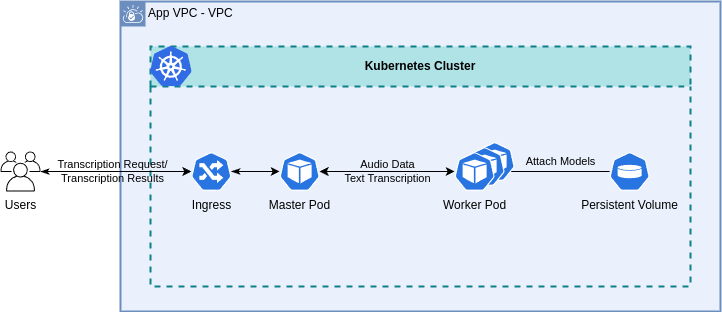
\includegraphics[width=\textwidth]{figures/previous_architecture.drawio.png}
    \caption{Previous Architecture of the ASR System}
    \label{fig:previous_architecture}
\end{figure}

\section{Challenges and Limitations}\label{section:challenges}
Previous Final Year Project (FYP) students have contributed to various aspects of this ASR system, such as deploying it on AWS with Terraform \cite{song_yu, kai_shern} and enhancing its security \cite{putra}. However, several significant limitations persists:
\begin{enumerate}
    \item \textbf{Tight Coupling:} The master and worker pods are tightly integrated, communicating synchronously via WebSocket connections. This restricts scalability, as components are highly dependent on each other, making it difficult to scale individual services independently \cite{tight_couple}.
    \item \textbf{Stateful Components:} Both the master and worker pods maintain state information, such as audio data and worker statuses. This reliance on stateful components complicates fault handling and exacerbates the system's lack of fault tolerance.
    \item \textbf{Worker Failures:} Worker pods can fail due to various reasons, including resource exhaustion, node crashes, or network disruptions. These failures leave audio processing tasks incomplete, disrupting the service. More importantly, worker failures directly impact the system’s ability to meet its Service Level Objectives (SLOs), particularly in terms of latency and availability.
    \item \textbf{Single Point of Failure:} The system relies on a single master pod, creating a single point of failure. If this pod crashes, there is no backup instance to handle requests, leading to potential service outages.
    
\end{enumerate}

\section{Project Scope}
The objective of this FYP is to enhance the scalability and resilience of the ASR system by transitioning to a decoupled architecture. The previous tightly coupled system struggled to handle fluctuating workloads and maintain service continuity during failures. To address these challenges, this project focuses on redesigning system components, improving scalability mechanisms, and enhancing failure recovery strategies.

\subsection{In Scope}
The project will address the following key areas:
\begin{enumerate}
    \item \textbf{Decoupling System Components with a Message Queue:} Introduce RabbitMQ as a message queue to facilitate asynchronous communication between the master and workers, enabling independent scaling and improves system fault tolerance.
    \item \textbf{Externalize State Management} Offload state management to Redis and RabbitMQ, reducing dependency on stateful components and enhancing overall system fault tolerance.
    \item \textbf{Developing a Dynamic and Predictive Scaling Policy for Workers:} Implement a dynamic scaling policy for worker pods that adjusts the number of instances based on real-time system load, ensuring optimal resource utilization and responsiveness.
    \item \textbf{Designing Mechanisms to Minimize Latency During Worker Failures:} Develop fault detection and recovery mechanisms to quickly identify and recover from worker failures, minimizing service disruptions and maintaining low latency.
    \item \textbf{Automatic Scaling of Master Pods:} Deploy multiple master pods with autoscaling capabilities based on CPU and memory usage, ensuring efficient allocation of resources under varying workloads.
\end{enumerate}

\subsection{Out-of-Scope}
While this project focuses on improving the system’s architecture and scalability, the following areas are beyond its scope:
\begin{itemize}
    \item \textbf{Modifications to the ASR Model:} The underlying speech recognition model used for transcription will remain unchanged. Enhancements to its accuracy, multilingual capabilities, or computational efficiency are beyond the project's focus.
    \item \textbf{Security Enhancements:} Although security is a critical aspect of any system, improvements such as encryption mechanisms, authentication, and access controls will not be covered in this research.
    \item \textbf{Monitoring and Observability:} While system performance will be evaluated, the project does not aim to build comprehensive logging, monitoring, or alerting frameworks beyond what is required for testing scalability and fault tolerance.
\end{itemize}

\section{Significance and Contributions}
This project significantly enhances the scalability, reliability, and fault tolerance of the ASR system, ensuring its availability under high-load conditions and unexpected failures. The improvements directly benefit NTU Speech Lab’s research initiatives and support critical applications such as SCDF’s emergency call centers, where real-time transcription is essential. 

By addressing the limitations of the existing architecture, this project makes the following key contributions:

\begin{enumerate}
    \item \textbf{Decoupled System Architecture:} Introduced RabbitMQ as a message queue to enable asynchronous communication between system components, allowing independent scaling of Workers and improving overall system robustness.
    
    \item \textbf{Dynamic and Predictive Worker Scaling:} Implemented an adaptive scaling policy for worker pods, dynamically adjusting the number of instances based on real-time system load to optimize resource utilization and responsiveness.

    \item \textbf{Automatic Scaling of Master Pods:} Configured autoscaling for master pods and other components based on CPU and memory consumption, ensuring efficient resource allocation.

    \item \textbf{Enhanced Fault Recovery Mechanisms:} Developed mechanisms for rapid detection and recovery of failed worker pods, reducing transcription disruptions and maintaining low-latency processing.

    \item \textbf{State Management with Redis:} Externalized application state management to Redis, reducing reliance on stateful components and improving resilience against crashes.

    \item \textbf{Deployment on Kubernetes with AWS:} Deployed the ASR system on Kubernetes clusters hosted on AWS, leveraging infrastructure-as-code tools like Terraform to streamline setup.

    \item \textbf{Refactored Codebase for Maintainability:} Restructured and modularized the existing codebase to align with the new architecture, enhancing maintainability, extensibility, and developer onboarding.

    \item \textbf{Comprehensive System Documentation:} Provided detailed documentation on system architecture, functionality, and key components to facilitate future development, troubleshooting, and maintenance.
\end{enumerate}


\section{Report Organisation}
This report is structured into five chapters, each focusing on a specific aspect of the project:

\begin{itemize}
    \item \hyperref[chapter:introduction]{\textbf{Chapter 1: Introduction}} - This chapter provides an overview of the project, including its background, importance, objectives, scope, and significance.
    
    \item \hyperref[chapter:literature_review]{\textbf{Chapter 2: Literature Review}} - This chapter introduces the relevant technologies used in the project and reviews previous FYP works on the ASR system.
    
    \item \hyperref[chapter:analysis_and_design]{\textbf{Chapter 3: Analysis and Design}} - This chapter presents an analysis of the current ASR system architecture and identifies its limitations. It then describes the proposed decoupled architecture, including the use of message queues and dynamic scaling policies.
    
    \item \hyperref[chapter:detailed_implementation]{\textbf{Chapter 4: Detailed Implementation}} - This chapter provides a detailed implementation of the new architecture, the development of the dynamic scaling policy, and the mechanisms implemented to handle worker failures.
    
    \item \hyperref[chapter:conclusion_and_future_work]{\textbf{Chapter 5: Conclusion and Future Work}} - This chapter summarizes the contributions of the project. It also outlines potential areas for future research and development to further improve the ASR system.
\end{itemize}


\chapter{Literature Review} \label{chapter:literature_review}
The development of reliable and scalable Automatic Speech Recognition (ASR) systems requires an understanding of modern distributed systems technologies and architectural design. This literature review examines the technologies and approaches relevant to enhancing ASR system scalability and resilience. The review begins with an introduction to the key technologies in distributed systems, containerization cloud infrastructure, chaos enginnering and message queues. It then discussed the previous work on the ASR system and explore the research gap.

\section{Distributed Systems Architecture}
\subsection{Evolution of Microservices}
The transition from monolithic to microservices architecture represents a fundamental shift in distributed systems design. Newman \cite{newman} defines microservices as small, autonomous services that work together, focusing on modularity and independent deployability. This architectural style has gained prominence due to its ability to support scalability, maintainability, and team autonomy \cite{microservices_benefits}. In the context of ASR systems, microservices architecture enables independent scaling of components and improved fault isolation.

\subsection{gRPC in Modern Applications}
gRPC is a high-performance Remote Procedure Call (RPC) framework \cite{grpc} that has significantly advanced service-to-service communication. It leverages Protocol Buffers, a language-agnostic interface definition language \cite{protocol_buffers}, enabling seamless communication between services written in different programming languages. This is particularly beneficial in microservices architectures, where different teams may develop services using diverse technology stacks. 

Performance analyses by Niswar et al. \cite{grpc_comparison} demonstrate that gRPC outperforms REST APIs and GraphQL in response time for retrieving both flat and nested data while also exhibiting lower CPU utilization. These advantages make gRPC particularly well-suited for ASR systems, where efficient, low-latency communication between components is crucial.

\subsubsection{gRPC Architecture}

Figure \ref{fig:grpc} illustrates the gRPC architecture, which consists of the following key components:
\begin{enumerate}
    \item \textbf{Client}: The application that initiates gRPC calls.
    \item \textbf{Server}: The application that implements the gRPC service and processes incoming requests.
    \item \textbf{Protocol Buffers}: A language-agnostic schema used to define services and message structures.
    \item \textbf{gRPC Stub}: The auto-generated client and server code derived from Protocol Buffer definitions.
    \item \textbf{HTTP/2}: The transport protocol used to facilitate efficient and multiplexed communication.
\end{enumerate}

\begin{figure}[H]
    \centering
    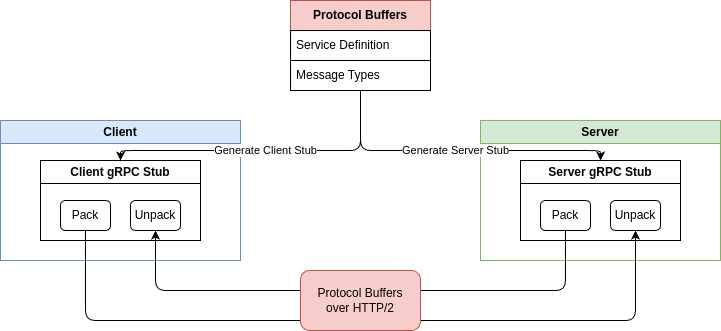
\includegraphics[width=\textwidth]{figures/gRPC_architecture.drawio.png}
    \caption{gRPC Architecture}
    \label{fig:grpc}
\end{figure}

\subsubsection{gRPC Communication Process}
The process begins with defining the service and message types using Protocol Buffers \cite{protocol_buffers_overview}. The \texttt{protoc} compiler then generates the client and server code. The client application uses the generated client stub to make a gRPC call \cite{grpc_api}, sending a request over HTTP/2 \cite{grpc_http2}. The server application uses the generated server stub to handle the gRPC call, processes the request, and sends back a response  over HTTP/2 \cite{grpc_api}.


\section{Containerization}
\subsection{Docker}
Docker is a service that leverages on operating system level virtualisation to package software into containers \cite{docker_definition}. Bernstein \cite{Bernstein} explains how Docker containers package applications with their dependencies. This consistency is crucial for ASR systems, where complex model and service dependencies must be managed effectively.

\subsection{Kubernetes}
Kubernetes is a container orchestration tool used to automate the deployment and management of containers \cite{k8s_definition}. 

A Kubernetes cluster (Figure \ref{fig:kubernetes_architecture}) contains the following key components \cite{k8s_cluster}:
\begin{enumerate}
    \item \textbf{Control Plane}: Manages the cluster and schedules workloads.
    \begin{itemize}
        \item \textbf{API Server}: Exposes the Kubernetes API.
        \item \textbf{etcd}: Key-value store for cluster data.
        \item \textbf{Scheduler}: Assigns workloads to nodes.
        \item \textbf{Controller Manager}: Ensures the desired state of the cluster.
        \item \textbf{Cloud Controller Manager}: Integrates with cloud provider APIs.
    \end{itemize}
    \item \textbf{Worker Nodes}: The compute nodes that run containerized applications.
    \begin{itemize}
        \item \textbf{Kubelet}: Agent that manages the node and communicates with the control plane.
        \item \textbf{Container Runtime}: Software that runs containers.
        \item \textbf{Kube Proxy}: Manages network connectivity.
    \end{itemize}
\end{enumerate}

\begin{figure}[H]
    \centering
    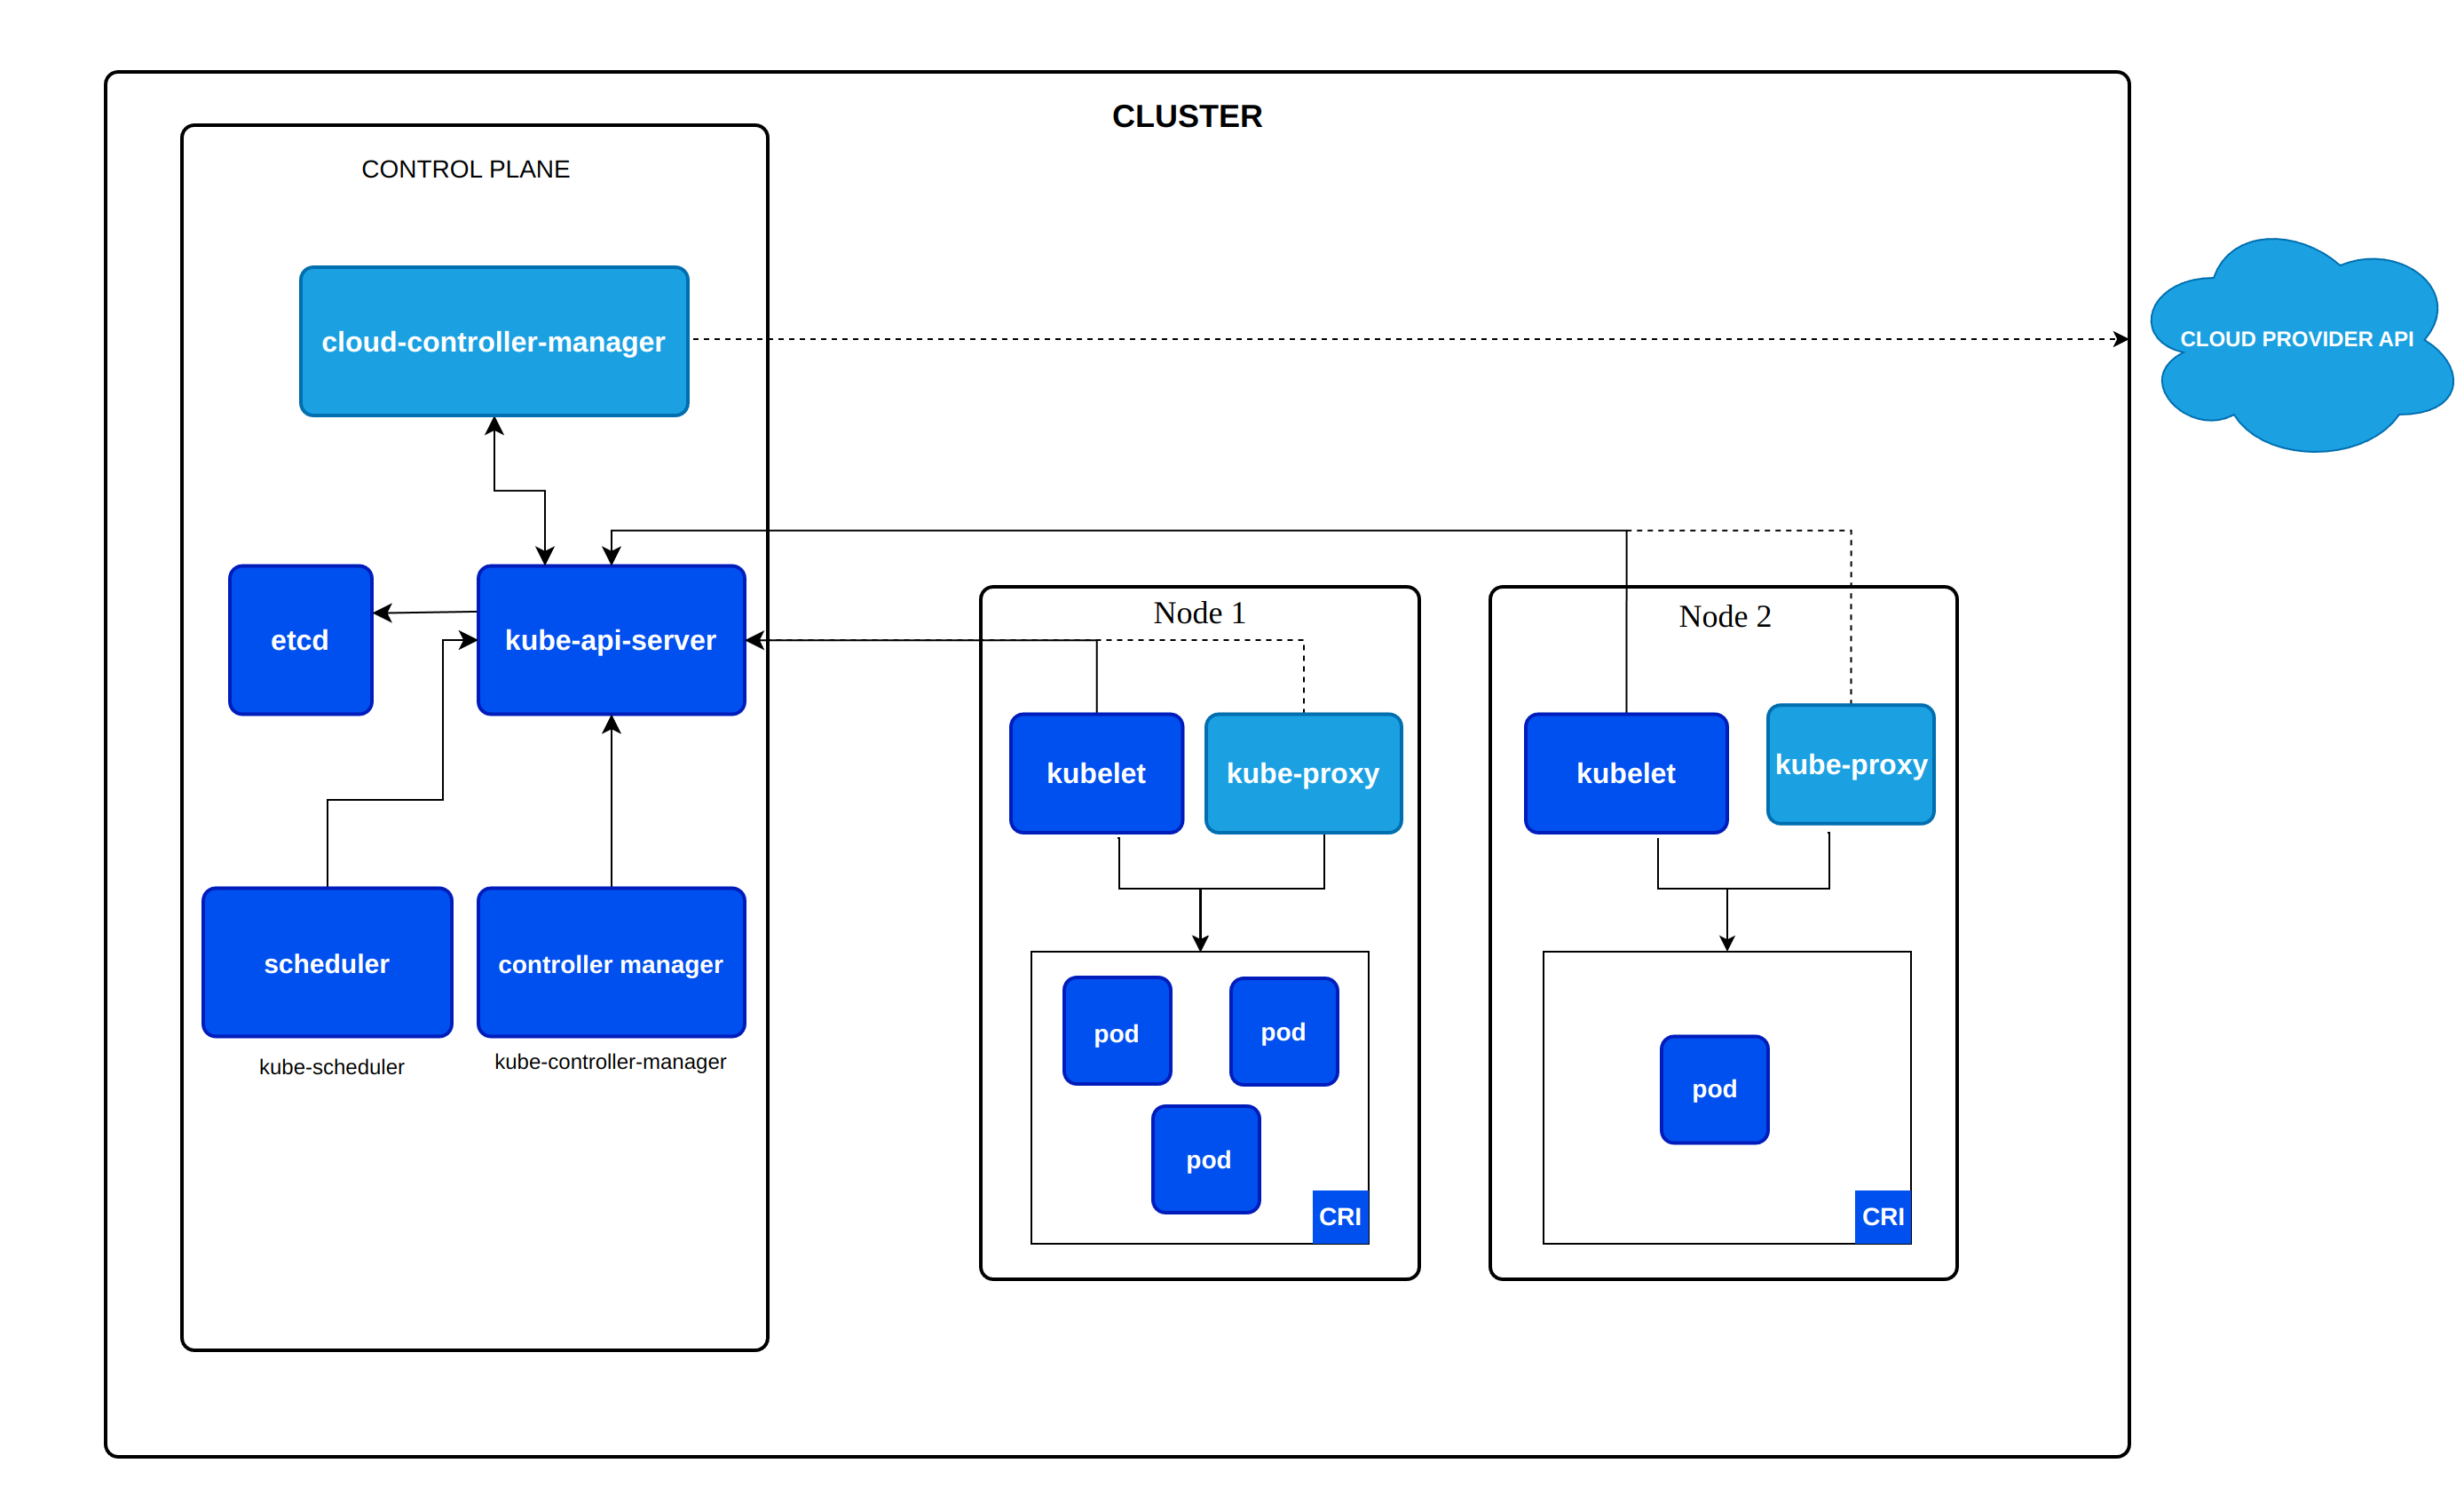
\includegraphics[width=\textwidth]{figures/kubernetes_architecture.png}
    \caption{Kubernetes Cluster Architecture \cite{k8s_cluster}}
    \label{fig:kubernetes_architecture}
\end{figure}

Burns et al. \cite{k8s_architecture} detail its architecture and ability to manage containerized applications at scale. For ASR systems, Kubernetes provides essential features such as automatic scaling, self-healing, and rolling updates \cite{k8s_features}, which are crucial for maintaining service reliability.

\subsection{Helm}
Helm is a package manager for Kubernetes applications \cite{helm_definition}. Helm utilises Charts, as reusable packages that contains pre-configured Kubernetes resources \cite{helm_charts}, making complex application deployments more manageable. These Charts function as templates that can be customized through value files \cite{helm_definition}, enabling environment-specific configurations while maintaining consistency in the underlying architecture.

\section{Amazon Web Services (AWS)}
AWS is a cloud service provider that offers a wide range of products and services. These services span compute, storage, networking, database, and container management, among others \cite{aws_definition}.

\subsection{Virtual Private Cloud (VPC)}
Amazon VPC forms the networking foundation for AWS resources, providing an isolated virtual network environment in the cloud \cite{vpc}. It enables users to define network architecture with custom IP address ranges, subnets, and routing tables \cite{vpc}. A key feature is its ability to span multiple Availability Zones (AZs) within a region, enhancing system resilience through geographical distribution \cite{vpc_az}.

\subsection{Elastic Compute Cloud (EC2)}
Amazon EC2 is a computing service that provides scalable virtual machines (instances) in the cloud \cite{ec2_definition}. It offers a wide range of instance types optimized for different use cases, from compute-intensive applications to memory-intensive workloads \cite{ec2_instance_types}. EC2 instances can be launched across multiple AZs for high availability. EC2 pricing models including on-demand, reserved, and spot instances to optimize costs based on workload patterns \cite{ec2_pricing}.

\subsection{Identity and Access Management (IAM)}
IAM provides fine-grained access control to AWS resources \cite{iam_definition}. It implements the principle of least privilege through a comprehensive policy framework that defines who (principal) can do what (actions) on which resources under specific conditions \cite{iam_security}. IAM enables organizations to manage user identities, roles, and permissions centrally, ensuring secure access to cloud resources while maintaining compliance requirements.

\subsection{Elastic Kubernetes Service (EKS)}
Amazon EKS is a managed Kubernetes service that simplifies the deployment, management, and scaling of containerized applications \cite{eks_definition}. It automatically manages the availability and scalability of the Kubernetes control plane across multiple AZs \cite{eks_definition}. EKS integrates seamlessly with other AWS services and supports various deployment models, including hybrid architectures that span cloud and on-premises environments \cite{eks_deployment}.

\subsection{Elastic Container Registry (ECR)}
Amazon ECR is a managed container registry service that simplifies the storage, management, and deployment of container images \cite{ecr_definition}. It provides encrypted image storage and integrates with AWS IAM for access control \cite{ecr_iam}. ECR features automatic image scanning for vulnerabilities \cite{ecr_image_scanning} and lifecycle policies for image management \cite{ecr_lifecycle}, making it an essential component in container-based architectures.

\subsection{Elastic File System (EFS)}
Amazon EFS provides scalable, fully managed network file storage for use with AWS cloud services and on-premises resources \cite{efs_definition}. Supporting the Network File System version 4 (NFSv4) protocol \cite{efs_work}, EFS can be accessed concurrently by thousands of compute instances \cite{efs_performance}. It automatically scales throughput when files are added or removed \cite{efs_performance}, making it ideal for applications requiring shared file access across multiple instances or containers.

\subsection{Elastic Block Store (EBS)}
Amazon EBS is a block storage service that is highly performant and scalable \cite{ebs_definition}. It can be used with EC2 instances to provide persistent storage volumes for EKS \cite{ebs_with_eks}. EBS volumes support various types, including General Purpose SSD (gp2), Provisioned IOPS SSD (io1), and Throughput Optimized HDD (st1) \cite{ebs_types}, enabling users to select the appropriate storage type based on performance requirements.

\section{Infrastructure-as-Code (IaC)}
IaC is an approach to managing and provisioning computing infrastructure through  configuration files, rather than through physical hardware configuration or interactive configuration tools. This method allows for the automation of infrastructure setup, ensuring consistency and reducing the risk of human error \cite{iac_benefits}.

\subsection{Terraform}
Terraform is an IaC tool that allows for the declarative management of cloud resources \cite{terraform_hashicorp}. This means that we define the desired final state of our architecture, and Terraform will apply changes only when necessary to achieve that state \cite{terraform_declarative}. Unlike traditional manual deployment through cloud provider consoles (often referred to as "ClickOps" \cite{clickops}), Terraform enables organizations to define their infrastructure using declarative configuration files. This code-driven approach transforms infrastructure deployment from a manual, error-prone process into an automated, version-controlled workflow.

Terraform enables teams to consistently replicate environments across development, testing, and production stages \cite{iac_benefits}, ensuring that infrastructure configurations remain identical at each phase. By maintaining infrastructure as code, teams can version control their changes, enabling peer reviews and the ability to roll back modifications if issues arise. Terraform also manages dependencies between different cloud resources automatically \cite{terraform_dependencies}, reducing the complexity of infrastructure deployment. 

\section{Chaos Engineering}
Chaos engineering is an approach to deliberately introducing failures to identify weaknesses and improve resilience \cite{chaos_engineering_definition}. By simulating conditions like Kubernetes pod failure, network delay, and node stress \cite{chaos_mesh_feature}, chaos engineering helps us observe system behaviour under stress and improve system robustness \cite{chaos_engineering_definition}. It also enhances incident response time by enabling a better understanding of failure scenarios \cite{chaos_engineering_definition}. Some chaos engineering tools include Chaos Mesh \cite{chaos_mesh_introduction} and AWS Fault Injection Simulator (FIS) \cite{fis_introduction}.

\section{In-memory Data Storage}
\subsection{Redis}
Redis is a high-performance, in-memory data store commonly used as a cache and a key-value database \cite{redis_definition}. Redis is fast, and thus well-suited for use in ASR systems, where it can store session information and temporary transcription data. This enables rapid access to frequently used data and facilitates reliable state management, ensuring smooth and responsive system performance. 

To achieve high availability, Redis can be configured with replication to keep it in sync with the primary instance \cite{redis_replication}. Redis Sentinel can be used to monitor Redis instances and perform automatic failover in case of primary instance failure \cite{redis_sentinel}. A group of Redis instances can be configured to be in sentinel mode, which can detect the failure of the primary Redis instance through a quorum and promote a replica to the primary (Figure \ref{fig:redis_sentinel}).

\begin{figure}[H]
    \centering
    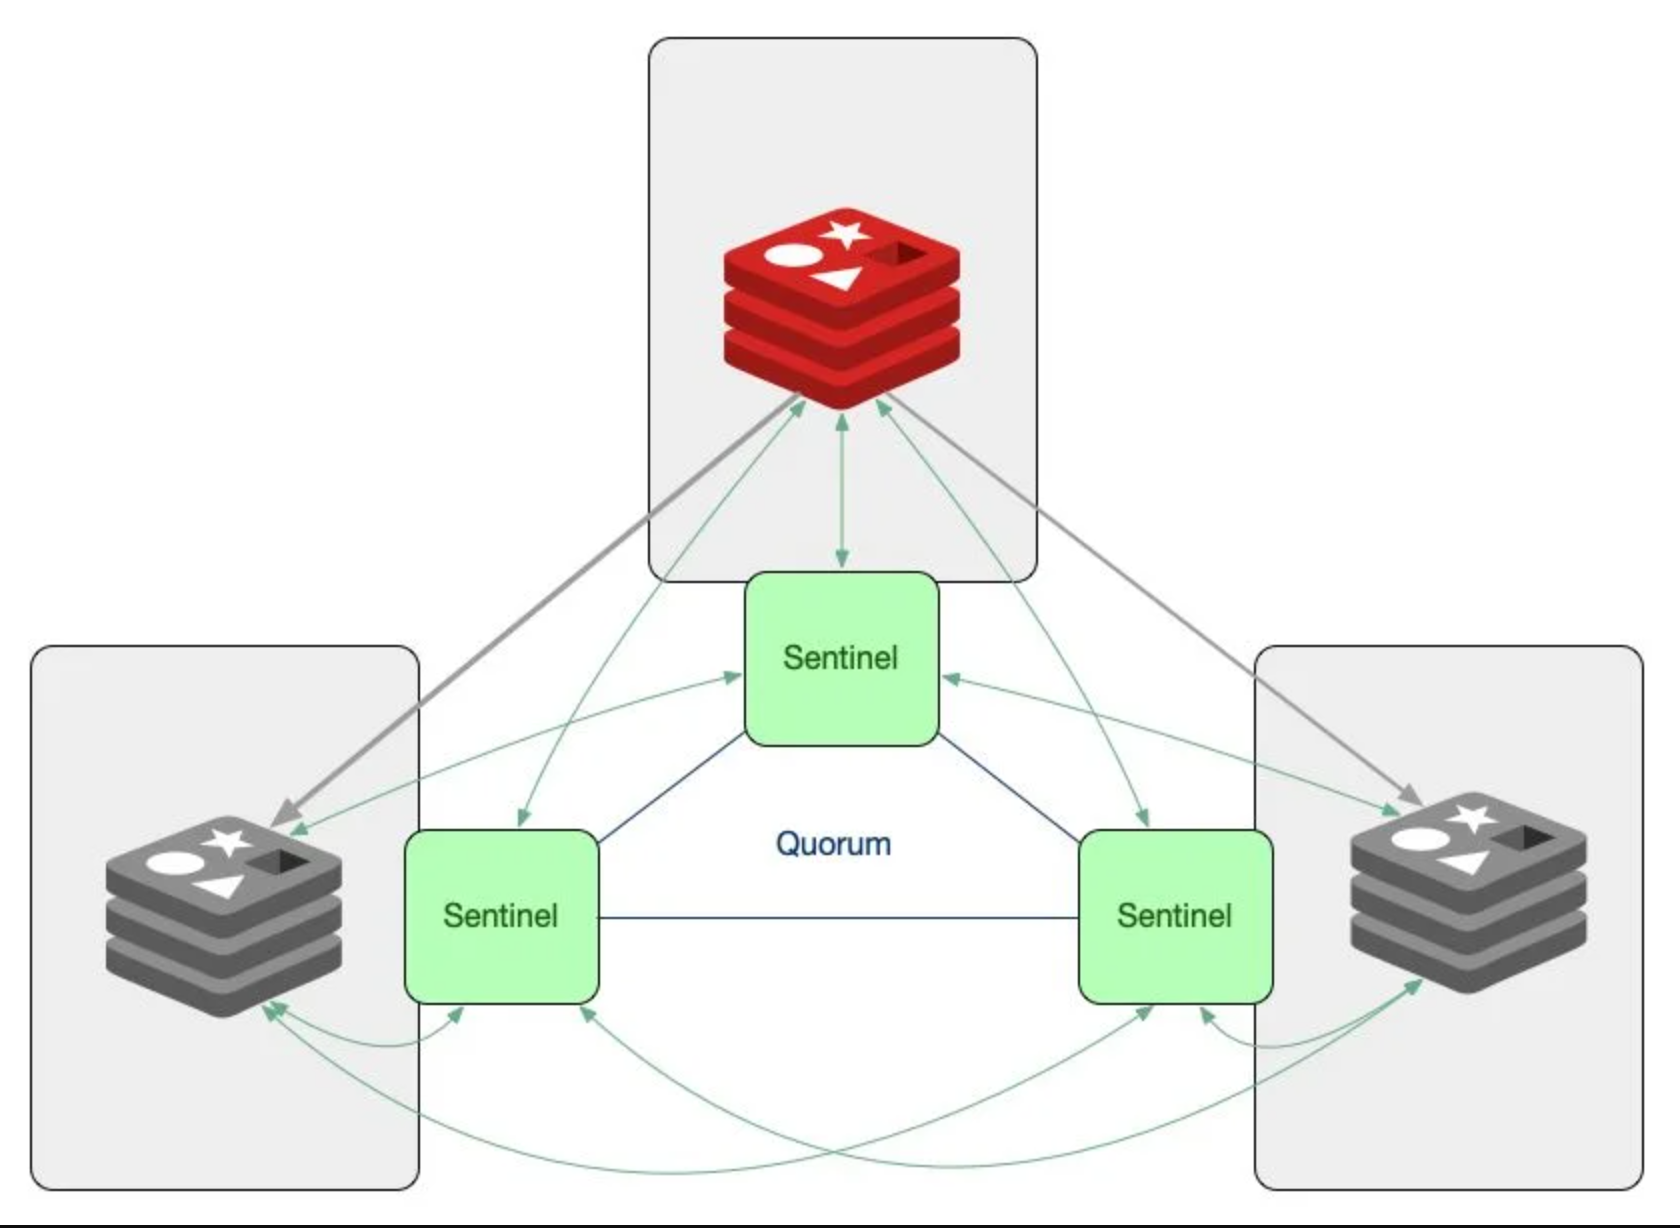
\includegraphics[width=0.8\textwidth]{figures/redis_sentinel.png}
    \caption{Redis Sentinel}
    \label{fig:redis_sentinel}
\end{figure}

\section{Message Queues}
Message queues enable asynchronous communication between services in distributed systems, providing temporary message storage and reliable delivery mechanisms \cite{queue_definition}. This asynchronous pattern facilitates decoupling of producers and consumers \cite{queue_decouple}, allowing components to scale independently and operate without direct dependencies on each other. 

\subsection{Apache Kafka}
Apache Kafka is designed as a distributed log-based messaging system, and its main use case is for ingesting and streaming real-time data \cite{kafka_definition}. Kafka's architecture centers around append-only logs (topics) divided into partitions, where messages are immutably stored and accessed via offset-based positioning \cite{kafka_documentation}.

\subsection{RabbitMQ}
RabbitMQ implements the Advanced Message Queuing Protocol (AMQP) \cite{rabbitmq_protocols} and operates as a broker-based message queue \cite{rabbitmq_definition}. It provides sophisticated message routing capabilities through exchanges and queues, supporting various patterns including publish-subscribe, and request-reply communications \cite{rabbitmq_routing}. RabbitMQ offers features such as message acknowledgments, dead letter queues, and priority queuing \cite{rabbitmq_routing}, making it particularly suitable for complex message routing requirements.

\subsection{Comparison of Kafka and RabbitMQ}
While both systems are robust message brokers, their architectural differences significantly impact their suitability for ASR applications. Below, we compare Kafka and RabbitMQ across key dimensions relevant to ASR systems.

\subsubsection{Message Ordering}
Kafka's partitioned architecture, while enabling high throughput, cannot guarantee message ordering across partitions. Dobbelaere and Esmaili \cite{kafka_v_rabbitmq} note that Kafka's ordering guarantees are limited to individual partitions.

RabbitMQ, through its queue-based architecture, maintains strict FIFO (First-In-First-Out) ordering within queues in the same channel \cite{kafka_v_rabbitmq}, making it more suitable for ASR systems where speech context and sequence are crucial.

\subsubsection{Message Delivery Guarantees}
Kafka provides at-least-once delivery semantics through offset management \cite{kafka_v_rabbitmq}, but consumers must handle offset commits carefully to avoid message reprocessing.

RabbitMQ's acknowledgment mechanism offers more flexible delivery guarantees, with built-in support for message acknowledgment \cite{kafka_v_rabbitmq} and automatic requeuing of unprocessed messages \cite{rabbitmq_nack}.

\subsubsection{Processing Requirements}
For ASR systems, where maintaining speech context is paramount \cite{speech_context}, RabbitMQ's single-queue consumer model aligns better with the need for sequential processing for live transcription tasks.

The research shows that while Kafka's throughput advantage is significant for high-volume streaming \cite{kafka_v_rabbitmq}, this benefit is less relevant for ASR workloads where processing speed is typically bounded by the speech recognition models rather than message throughput.

\subsubsection{Message Queue Selection} \label{subsection:research_gap}
Based on these considerations and supported by Dobbelaere and Esmaili's \cite{kafka_v_rabbitmq} findings, RabbitMQ emerges as the more appropriate choice for ASR systems due to its strong message ordering guarantees, flexible acknowledgement mechanisms, and support for sequential processing requirements. By leveraging RabbitMQ's features, ASR systems can ensure accurate transcription results and maintain the context of speech data for live transcription throughout the processing pipeline.



\section{Previous Work}
Putra \cite{putra} had worked on the same ASR system and his project effectively highlights the advantages of transitioning from a tightly coupled ASR system to a decoupled microservices architecture using Apache Kafka. The use of Kubernetes and other modern cloud-native tools such as Kyverno, Falco, and Knative demonstrates a robust effort to address scalability, reliability, and security challenges in ASR systems. The project discusses the integration of Kafka as the message broker to decouple the master and worker components, ensuring fault tolerance and enabling the system to recover from worker crashes without losing data.

\subsection{Research Gap}
A significant research gap exists in the implementation's choice of message broker technology. The selection of Kafka for the ASR system raises concerns regarding its fit for scenarios requiring high data accuracy and context preservation. While Kafka's high throughput and durability are valuable for many systems, ASR workflows are fundamentally bottlenecked by the processing speed of workers, not the message broker. This mismatch between technology choice and system requirements suggests that RabbitMQ would be a more suitable alternative due to its task-oriented features and built-in support for state-dependent processing, which better aligns with the sequential nature of speech processing tasks.

Furthermore, while Putra’s work \cite{putra} demonstrated promising results, a practical limitation emerged as the research team no longer has access to his project's codebase. This circumstance has created an opportunity to revisit the system's architecture with fresh perspective, particularly in the areas of component decoupling and scaling mechanisms. The current project therefore aims to not only address the technological fit of the message broker but also to establish a well-documented implementation that can be maintained and evolved by the research team.


\chapter{Analysis and Design Approach} \label{chapter:analysis_and_design}
\section{Previous Architecture}
The previous architecture of the ASR system, as illustrated in Figure \ref{fig:previous_architecture}, was deployed on a Kubernetes cluster hosted on AWS.

Transcription requests were routed through an NGINX Ingress Controller, which forwarded them to a Master Pod responsible for managing transcription tasks. Upon receiving a request, the Master Pod authenticated it and, if a worker Pod was available, initiated a WebSocket connection. The audio data was then transmitted to the worker Pod for transcription.

Each Worker Pod was associated with a model attached via a Persistent Volume Claim (PVC). After processing, the Worker Pod sent the transcription results back to the Master Pod, which then forwarded them to the client.

\section{Challenges and Design Evolution}
Based on the evaluation of the previous architecture, several challenges were identified. The new design addresses these by adopting a more decoupled, scalable, and fault-tolerant approach.

\subsection{Decoupling Master and Worker Pods}
The reliance on synchronous WebSocket communication between the Master and Worker Pods introduced significant challenges in fault tolerance and scaling. Any failure in either component would disrupt ongoing transcription tasks. Additionally, scaling Worker Pods dynamically was constrained direct communication.

\subsubsection{Proposed Solution: Asynchronous Messaging}
To enhance scalability and resilience, the new architecture adopts an message queue approach using RabbitMQ (Figure \ref{fig:decouple}).
\begin{figure}[!ht]
    \centering
    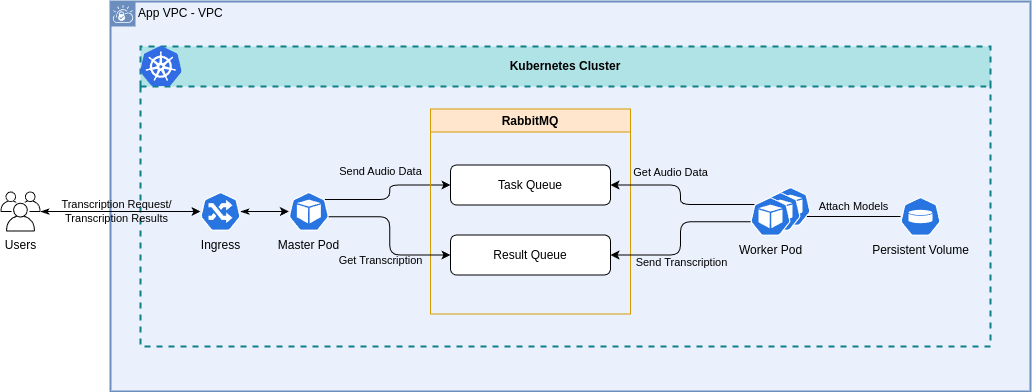
\includegraphics[width=\textwidth]{figures/decouple.drawio.png}
    \caption{Decoupling the Master and Worker Pods}
    \label{fig:decouple}
\end{figure}

In the new design, the Master Pod publishes transcription tasks to a RabbitMQ task queue. Worker Pods asynchronously consume tasks, process the audio, and publish results to a results queue. The Master Pod retrieves transcription results and sends them back to the client.

This design eliminates direct dependencies between components, allowing independent scaling and improved fault tolerance. RabbitMQ was chosen over alternatives like Kafka due to its robust support for message acknowledgments, ensuring no transcription task is lost in case of failures.

\subsection{Enhancing State Management and Fault Tolerance}
Previously, the Worker Pods stored audio data in an in-memory queue. If a worker pod crashed, any buffered data was lost, requiring clients to retransmit. This dependency on volatile storage complicated recovery and degraded system reliability.

\subsubsection{Proposed Solution: Redis for State Persistence}
To mitigate data loss and improve fault tolerance, the application state is now stored in Redis, ensuring that if a service fails, it can recover essential state information. Additionally, RabbitMQ’s message durability ensures that queued transcription tasks are not lost if a worker crashes. If a worker pod fails mid-transcription, a new worker can pick up the task from the queue without requiring client intervention. This redesign significantly enhances fault tolerance and ensures a seamless recovery mechanism.

\subsection{Scaling and Load Management}
The previous deployment relied on a single master pod, creating a single point of failure. Additionally, worker scaling required manual intervention, making it inefficient and slow in responding to traffic fluctuations.

\subsubsection{Proposed Solution: Kubernetes Autoscaling and Worker Manager}
The new architecture incorporates:
\begin{itemize}
    \item \textbf{Kubernetes Horizontal Pod Autoscaler (HPA):} Automatically scales master pods based on request load, preventing service disruptions.
    \item \textbf{Dynamic Worker Scaling via Worker Manager:} A new Worker Manager service dynamically adjusts worker pod replicas based on configurable \texttt{SCALING\_TARGET} (See Code \ref{lst:worker_scaling}).
\end{itemize}

The dynamic scaling policy is managed by an additional service called the Worker Manager, which is described in detail in \hyperref[section:worker_manager]{\textit{Chapter 4: Detailed Implementation}}. The Worker Manager monitors the current state of worker pods for each model and adjusts the number of pods accordingly to maintain the scaling target.

Key features of this solution include:
\begin{itemize}
    \item \textbf{Load-based scaling:}  The Worker Manager scales worker pods up or down based on current traffic and processing load, ensuring optimal resource utilization.
    \item \textbf{Minimized scaling disruptions:}  To prevent excessive scaling activity, the scaling policy incorporates a configurable \texttt{CHECK\_INTERVAL} that limits the frequency of scaling operations.
\end{itemize}

\subsection{Improving Documentation and Code Readability}
The previous ASR system codebase lacked sufficient documentation, making it difficult to onboard new developers and troubleshoot issues. Without clear documentation, understanding system behavior and implementing new features was time-consuming.

\subsubsection{Proposed Solution: Structured Documentation Strategy}
To address these challenges, the new codebase will prioritize comprehensive and clear documentation. A detailed \texttt{README} file will provide an overview of the project, including its architecture, purpose, and key components. Additionally, inline comments will be incorporated throughout the codebase to explain the functionality and intent of each component.

This approach helps to onboard new developers faster, through providing them with more context to understand the system better. Additionally, it ensures maintainability by ensuring the developers can easily understand and modify the codebase in the future.

An inline comment explaining the purpose of a function or section of code can significantly improve readability. For instance, Code \ref{lst:code_documentation} shows an example of an inline comment that describes the purpose of a function and its parameters.

By integrating documentation and inline comments into the development process, the new codebase will improve the maintainability and quick onboarding of new developers.

\chapter{Detailed Implementation} \label{chapter:detailed_implementation}
This chapter provides an in-depth explanation of the design, architecture, and deployment of the newly implemented ASR system. It elaborates on the functionality of the system components and how they interact to achieve scalability, fault tolerance, and efficient processing.

\section{Architecture}
The new architecture of the ASR system is illustrated in Figure \ref{fig:new_architecture}. The system is designed with a microservices architecture, where each component is responsible for a specific task. 

The system consists of the following components:
\begin{itemize}
    \item \textbf{Client:} The frontend user interface that initiates transcription requests and receives the results.
    \item \textbf{NGINX Ingress Controller:} Routes incoming requests to the Live Processing Service.
    \item \textbf{Live Processing Service:} Formerly known as the Master Pod, it manages transcription tasks, coordinates worker allocation with the Worker Manager, and maintains a WebSocket connection with the client.
    \item \textbf{Worker Manager:} Allocates workers to process audio data based on the requested model and monitors the worker pods.
    \item \textbf{Worker:} Process the audio data using the specified ASR model and return the transcription results.
    \item \textbf{Message Queues:} RabbitMQ is used to decouple the communication between the Live Processing Service and the Worker.
    \item \textbf{Redis:} Stores the state information of the system, such as worker statuses and task details.
\end{itemize}

\begin{figure}[!h]
    \centering
    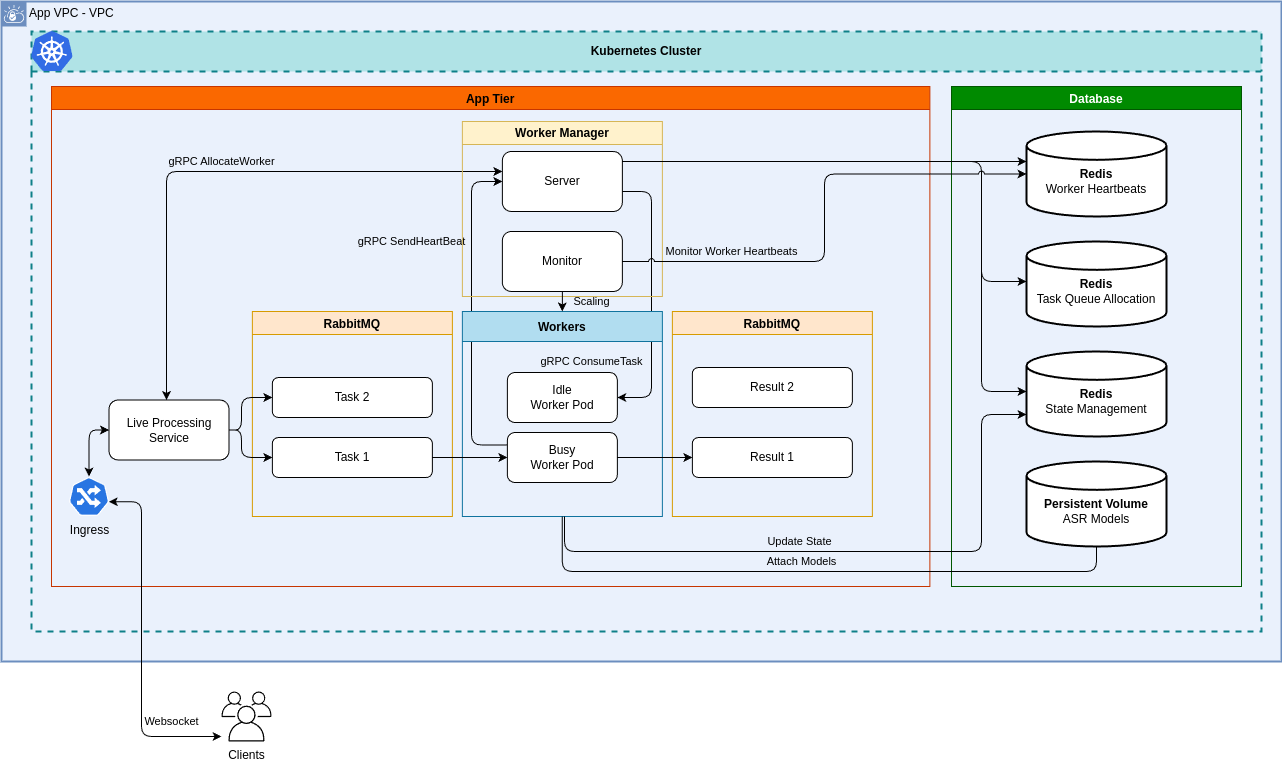
\includegraphics[width=\textwidth]{figures/new_architecture.drawio.png}
    \caption{New Architecture of the ASR System}
    \label{fig:new_architecture}
\end{figure}

\subsection{System Flow}
The sequence diagram in Figure \ref{fig:sequence_diagram} provides a detailed visualization of the ASR system's flow, showing the interactions between components during the transcription process.

\clearpage

\begin{figure}[ht]
    \centering
    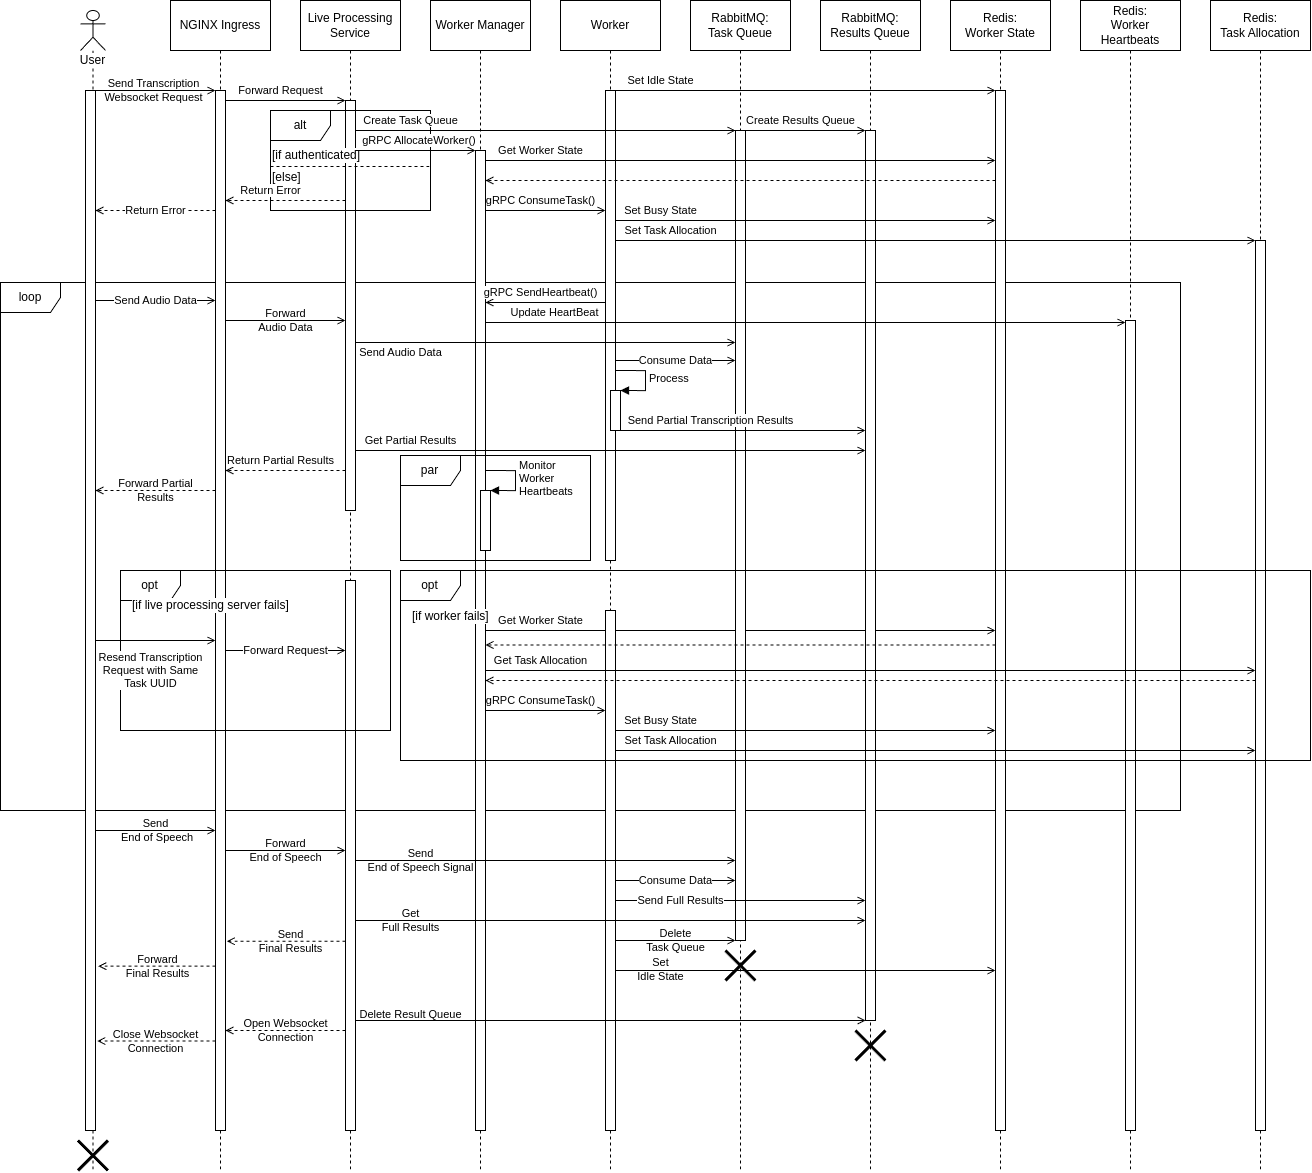
\includegraphics[width=\textwidth]{figures/sequence_diagram.drawio.png}
    \caption{Sequence Diagram of the ASR System}
    \label{fig:sequence_diagram}
\end{figure}

\subsubsection{Main Flow}
\begin{enumerate}
    \item The client establishes a WebSocket connection through the NGINX Ingress Controller to the Live Processing Service.
    \item Upon receiving the connection, the Live Processing Service creates two queues in RabbitMQ for each task:
    \begin{itemize}
        \item \texttt{task.<UUID of the task>}: Queue for the audio data to be processed.
        \item \texttt{result.<UUID of the task>}: Queue for the transcription results of the task.
    \end{itemize} 
    \item The Live Processing Service invokes the Worker Manager’s gRPC API to allocate a worker for the task.
    \item The Live Processing Service places audio data into the task queue.
    \item The Worker Manager checks the Redis database for an idle worker with the requested ASR model and assigns it to the task. The worker is notified via a gRPC call.
    \item The worker updates its state in Redis to \texttt{BUSY} and begins processing the audio data.
    \item Partial transcription results are sent to the result queue as the audio is processed.
    \item The Live Processing Service retrieves these partial results from the result queue and streams them back to the client via the WebSocket connection.
    \item Workers send periodic heartbeats to the Worker Manager to confirm their health status.
    \item When the client detects the end of speech, it notifies the Live Processing Service, which marks the task as complete by sending a special End of Speech (\texttt{EOS}) message to the task queue.
    \item Upon processing the \texttt{EOS} message, the worker updates its state in Redis to \texttt{IDLE} and sends the final transcription result to the result queue.
    \item The Live Processing Service retrieves the final result from the result queue and delivers it to the client via WebSocket.
    \item Once all results are delivered, the WebSocket connection is closed.
\end{enumerate}

\subsubsection{Worker Failure Flow}
To maintain fault tolerance, the system detects and recovers from worker failures as follows:
\begin{enumerate}
    \item The Worker Manager detects a failure when it stops receiving heartbeats from a worker.
    \item It gets a new idle worker with the same ASR model from Redis and reassigns the task to the new worker.
    \item The new worker retrieves the pending task from the task queue, updates its state to \texttt{BUSY}, and resumes processing the audio data.
\end{enumerate}

\subsubsection{Live Processing Service Server Failure Flow}
To handle failures of the Live Processing Service:
\begin{enumerate}
    \item The client reestablishes a WebSocket connection to the Live Processing Service and resends the transcription request using the same task UUID.
    \item The Live Processing Service uses the existing task and result queues to continue processing and retrieving results, ensuring no data is lost.
\end{enumerate}

\section{Live Processing Service}
The Live Processing Service manages WebSocket connections with clients to facilitate real-time transcription. Its primary functions include:
\begin{enumerate}
  \item \textbf{WebSocket Communication:} Establishing and managing WebSocket connections to stream transcription results in real time.
  \item \textbf{Task Management:} Creating and managing task and result queues in RabbitMQ for each transcription request.
  \item \textbf{Worker Allocation:} Requesting worker allocation from the Worker Manager based on the required ASR model.
\end{enumerate}


The Live Processing Service is built using Tornado \cite{tornado}, an asynchronous web framework optimized for handling long-lived connections and scaling to thousands of concurrent WebSocket sessions. This makes it well-suited for real-time applications such the ASR system.

\subsection{WebSocket Handler}
The WebSocket handler manages WebSocket connections with clients and streams transcription results back to them. It processes the following events:

\begin{itemize}
    \item \textbf{open:} Authenticates incoming WebSocket requests, initializes task and result queues in RabbitMQ, requests worker allocation from the Worker Manager, and starts consuming transcription results from the result queue.
    \item \textbf{on\_message:} Receives audio data from the client and places it into the task queue.
    \item \textbf{close:} Closes the WebSocket connection with the client and performs cleanup operations.
\end{itemize}

\subsection{Asynchronous RabbitMQ}
To maintain non-blocking performance, the Live Processing Service utilizes an asynchronous RabbitMQ client compatible with Tornado. This enables concurrent task management without disrupting the event loop.

A dedicated asynchronous RabbitMQ client with exponential backoff was implemented to handle network disruptions and RabbitMQ failures. Code \ref{lst:rabbitmq_client} illustrates the implementation.

\begin{lstlisting}[language=python, caption={Asynchronous RabbitMQ Client}, label={lst:rabbitmq_client}]
async def connect(self):
      """
      Connect to RabbitMQ.
      """
      attempts = 0
      while attempts < RABBITMQ_MAX_RETRIES:
          try:
              self.logger.info(f"trying to connect to {self.host}:{self.port}")
              self.logger.info(f"using {self.username} as username")
              self.connection = await aio_pika.connect_robust(
                  host=self.host,
                  port=self.port,
                  login=self.username,
                  password=self.password,
              )
              self.logger.info("Connected to RabbitMQ")
              break
          except Exception as e:
              self.logger.error(f"Failed to connect to RabbitMQ: {e}")
              attempts += 1
              await asyncio.sleep(RABBITMQ_BACKOFF_FACTOR * attempts)
\end{lstlisting}

\subsection{Worker Allocation via gRPC}
The Live Processing Service requests worker allocation from the Worker Manager using gRPC. This ensures low-latency, efficient communication, which is critical for real-time transcription.

To allocate a worker for a transcription task, the Live Processing Service sends a gRPC request specifying the required ASR model. The Worker Manager responds with an available worker instance. This interaction leverages Protocol Buffers for efficient data serialization and the gRPC stub generated from the service definition.

Code \ref{lst:grpc_request} illustrates the gRPC request process.

\begin{lstlisting}[language=python, caption={gRPC Request for Worker Allocation}, label={lst:grpc_request}]
async def allocate_worker_from_worker_manger(self, model_name, task_queue):
      """
      Allocate an idle worker from the WorkerManager service.

      Args:
          model_name (str): Name of the model to allocate the worker for.
          task_queue (str): Name of the task queue to assign to the worker.
      """
      async with grpc.aio.insecure_channel(
          f"{WORKER_MANAGER_SERVICE}:{WORKER_MANAGER_PORT}"
      ) as channel:
          stub = worker_manager_pb2_grpc.WorkerManagerServiceStub(channel)
          request = worker_manager_pb2.AllocateWorkerRequest(
              model_name=model_name, task_queue=task_queue
          )
          response = await stub.AllocateWorker(request)

          if response.success:
              logger.info(
                  f"Worker {response.worker_name} allocated successfully: {response.message}"
              )
              return response.worker_name
          else:
              logger.error(f"Failed to allocate worker: {response.message}")
              return None
\end{lstlisting}


\section{Worker}
The primary function of the Worker is to process audio data using the specified ASR model and return transcription results.  

Each Worker loads an ASR model developed by the NTU Speech Lab, which is based on the Kaldi ASR toolkit \cite{kaldi}. The model is loaded into memory at startup, enabling low-latency transcription of incoming audio data.

\subsection{Audio Processing}
Once the Worker Manager assigns an idle Worker to a task via gRPC, the Worker retrieves the audio data from the task queue in RabbitMQ. It then processes the audio using the ASR model and publishes the transcription results to the result queue in RabbitMQ.  

To facilitate fault tolerance, the Worker updates its state in Redis when processing a task. It marks itself as \texttt{busy} and records the assigned task. This allows the Worker Manager to track active tasks and reassign them if a Worker fails.

Figure \ref{fig:worker_processing} illustrates the flow of audio processing in the Worker.
\begin{figure}[ht]
  \centering
  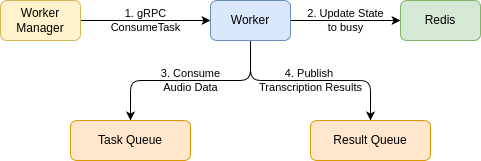
\includegraphics[width=.8\textwidth]{figures/worker_processing.drawio.png}
  \caption{Worker Processing Flow}
  \label{fig:worker_processing}
\end{figure}

\subsection{Heartbeat Monitoring}
To enable health monitoring, the Worker sends periodic heartbeat signals to the Worker Manager (Figure \ref{fig:worker_heartbeat}). These heartbeats allow the Worker Manager to detect failures and reallocate tasks accordingly. Further details on this mechanism are provided in Subsection \ref{subsection:worker_manager_monitor}.

\begin{figure}[ht]
  \centering
  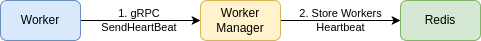
\includegraphics[width=.8\textwidth]{figures/worker_heartbeat.drawio.png}
  \caption{Worker Heartbeat Monitoring}
  \label{fig:worker_heartbeat}
\end{figure}

\section{Worker Manager} \label{section:worker_manager}
The Worker Manager is responsible for managing and coordinating worker pods to ensure efficient task processing and fault tolerance. Its core responsibilities include:
\begin{itemize}
  \item \textbf{Worker Allocation:} Assigning idle workers to process incoming audio data.
  \item \textbf{Health Monitoring:} Tracking worker health through periodic heartbeats.
  \item \textbf{Task Reassignment:} Detecting worker failures and reallocating tasks to maintain continuity.
  \item \textbf{Scaling Policy:} Dynamically adjusting the number of worker pods based on system load.
\end{itemize}


The Worker Manager consists of two primary components:
\begin{enumerate}
    \item \textbf{Worker Manager Server:} Exposes gRPC APIs for worker allocation and heartbeat monitoring.
    \item \textbf{Worker Manager Monitor:} Detects worker failures, reallocates tasks, and enforces scaling policies.
\end{enumerate}

\subsection{Worker Manager Server}

The Worker Manager Server provides two main gRPC endpoints (Code \ref{lst:worker_manager_server}):
\begin{enumerate}
    \item \texttt{AllocateWorker}: Assigns an idle worker to handle a given transcription task.
    \item \texttt{SendHeartbeat}: Receives periodic heartbeats from workers to track their health status. Stores the heartbeat timestamps in Redis for monitoring.
\end{enumerate}

Figure \ref{fig:worker_manager_server} shows how the Worker Manager Server interacts with the Live Processing Service, busy workers and Redis.

\begin{enumerate}
  \item [1] The Live Processing Service requests worker allocation via \texttt{AllocateWorker}.
  \item [2.1] The busy workers send periodic heartbeats to the Worker Manager Server via \texttt{SendHeartbeat}.
  \item [2.2] The Worker Manager Server then stores these heartbeat timestamps in Redis for monitoring.
\end{enumerate}

\begin{figure}[H]
  \centering
  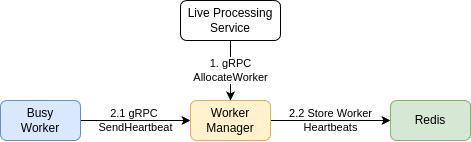
\includegraphics[width=.8\textwidth]{figures/worker_manager_server.drawio.png}
  \caption{Worker Manager Server Interaction}
  \label{fig:worker_manager_server}
\end{figure}


\subsection{Worker Manager Monitor} \label{subsection:worker_manager_monitor}
The Worker Manager Monitor is responsible for tracking worker health and handling task reallocation. It retrieves the latest heartbeat timestamps of workers from Redis. If a worker fails to send a heartbeat within a predefined timeout, it is considered unavailable, and its task is reassigned to another worker. This process is illustrated in Figure \ref{fig:worker_manager_monitor}.
\begin{figure}[ht]
  \centering
  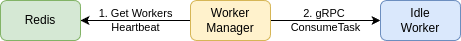
\includegraphics[width=.8\textwidth]{figures/worker_manager_heartbeat.drawio.png}
  \caption{Worker Manager Heartbeat Monitoring}
  \label{fig:worker_manager_monitor}
\end{figure}

Code \ref{lst:worker_fault_tolerance} shows the snippet of the Worker Manager Monitor's fault tolerance mechanism for the workers.

\begin{lstlisting}[language=python, caption={Worker Fault Tolerance Mechanism}, label={lst:worker_fault_tolerance}]
  async def monitor_heartbeats(self):
        """
        Monitor worker heartbeats and reallocate workers if necessary.
        """
        logger.info("Monitoring worker heartbeats...")
        self.redis_client = self.redis.get_client()
        while True:
            current_time = asyncio.get_event_loop().time()
            # logger.debug(f"Current time: {current_time}")
            for worker_name, value in self.redis_client.hgetall(
                "WorkerHeartbeats"
            ).items():
                lock_key = f"lock:worker_heartbeat:{worker_name}"
                try:
                    # Acquire distributed lock
                    if self.acquire_lock(lock_key):
                        model_name, last_heartbeat = value.split(",")
                        if (
                            current_time - float(last_heartbeat)
                            > WORKER_HEARTBEAT_TIMEOUT
                        ):
                            logger.info(
                                f"Worker {worker_name} missed heartbeat. Allocating new worker."
                            )
                            try:
                                task_queue = self.redis_client.hget(
                                    "TaskAllocation", f"Worker:{worker_name}"
                                )
                            except Exception as e:
                                logger.error(f"Failed to get task queue: {str(e)}")
                                raise
                            self.allocate_worker(model_name, task_queue)
                            self.redis_client.hdel("WorkerHeartbeats", worker_name)
                            logger.info(f"Worker {worker_name} deallocated.")
                    else:
                        logger.warning(f"Failed to acquire lock for {worker_name}")
                except Exception as e:
                    logger.error(
                        f"Failed to monitor heartbeat for {worker_name}: {str(e)}"
                    )
                finally:
                    # Release distributed lock
                    self.release_lock(lock_key)

            await asyncio.sleep(WORKER_MANAGER_MONITOR_INTERVAL)
\end{lstlisting}

To prevent race conditions when multiple Worker Manager pods are deployed, the Worker Manager first acquires a distributed lock before checking a worker’s last heartbeat. If a worker exceeds the timeout threshold, it is removed, and a new worker is assigned to its task queue.

\subsubsection{Testing Worker Fault Tolerance}
To validate the fault tolerance mechanism, the Worker Manager was tested under failure scenarios, such as unexpected worker crashes.

To simulate a worker failure, worker pod processing the audio data can be delibrately terminated using the following command:
\begin{verbatim}
  kubectl delete -n asr-sdk --now <worker-pod-name> \
    --cascade=background
\end{verbatim}

Figure \ref{fig:worker_fault_tolerance} illustrates the Worker Manager detecting that the worker pod \texttt{worker-\allowbreak stateful-english-0} has failed to send a heartbeat. As a result, it reallocates the task to an available idle worker, \texttt{worker-stateful-english-1}, ensuring uninterrupted processing.

\begin{figure}[H]
  \centering
  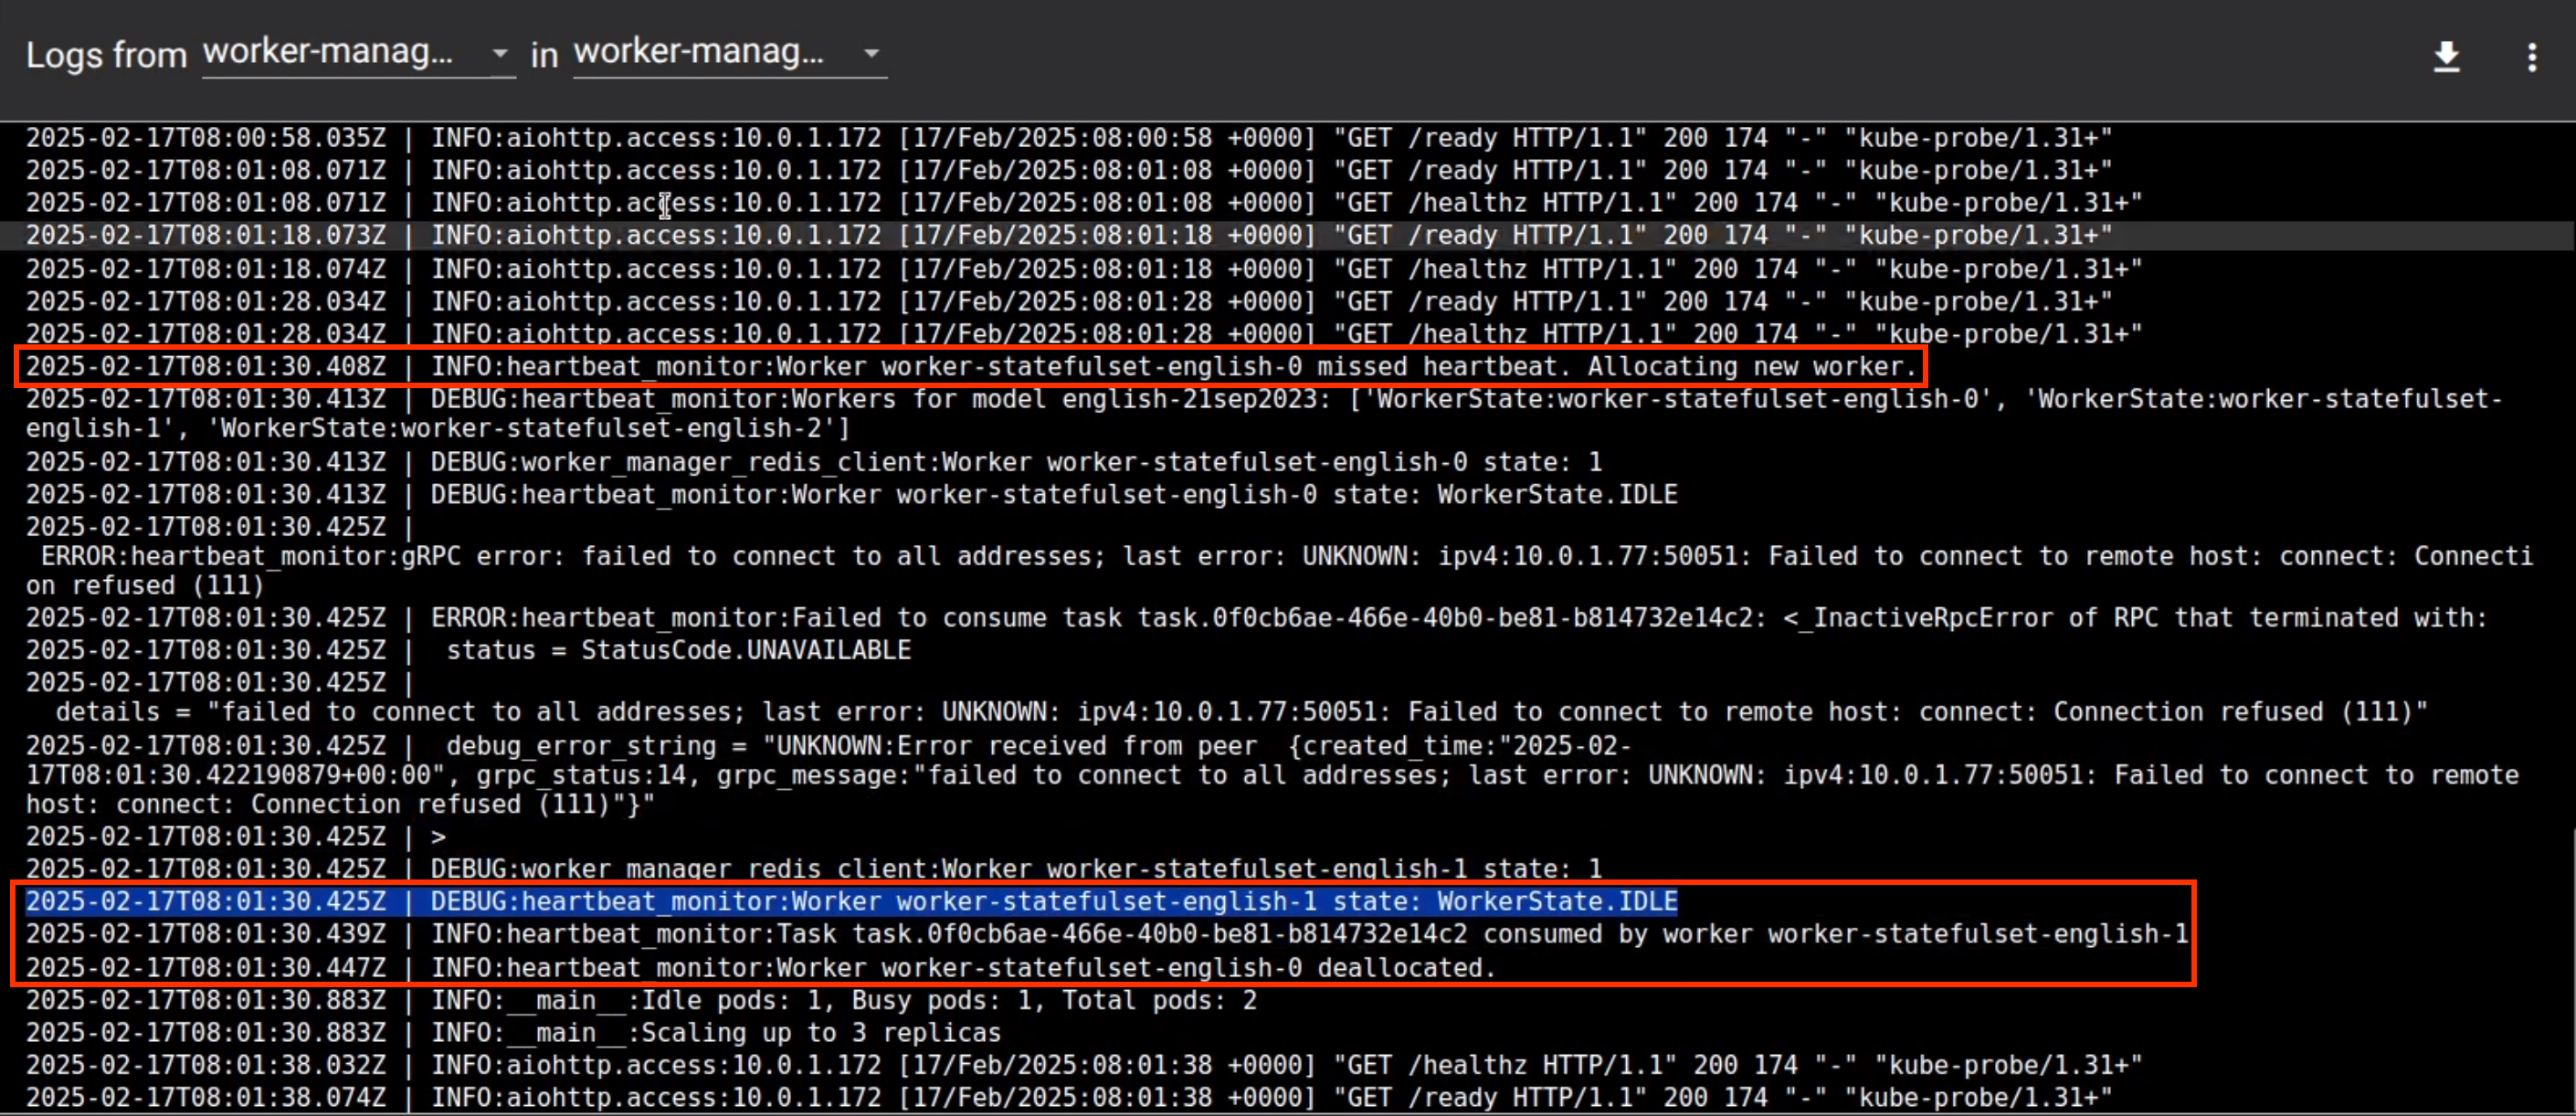
\includegraphics[width=\textwidth]{figures/worker_fault_tolerance.png}
  \caption{Worker Fault Tolerance Testing}
  \label{fig:worker_fault_tolerance}
\end{figure}

\subsubsection{Worker Scaling Policy}
The Worker Manager dynamically scales worker pods based on system load. A configurable threshold, \texttt{SCALING\_TARGET}, defines the minimum number of idle pods required at any given time. The Worker Manager periodically evaluates worker utilization and adjusts the number of replicas accordingly to ensure optimal resource allocation.

Figure \ref{fig:worker_scaling_policy} illustrates an example where there are 2 busy worker pods and 2 idle worker pods. If the \texttt{SCALING\_TARGET} is set to 3, the Worker Manager scales up the Worker StatefulSet to 5 replicas when the number of idle pods falls below the threshold. Conversely, when the workers finish processing, the Worker Manager scales down the replicas to ensure the number of idle pods meets the \texttt{SCALING\_TARGET}.

\begin{figure}[H]
  \centering
  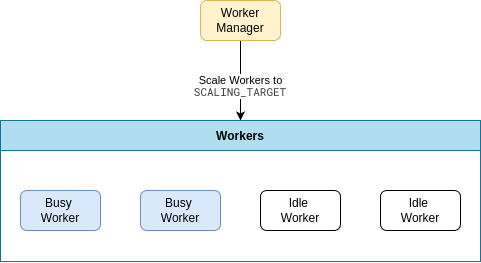
\includegraphics[width=.8\textwidth]{figures/worker_scaling_policy.drawio.png}
  \caption{Worker Scaling Policy Example}
  \label{fig:worker_scaling_policy}
\end{figure}

Code \ref{lst:worker_scaling} shows the snippet of the Worker scaling mechanism.

\begin{lstlisting}[language=python, caption={Worker Scaling Policy}, label={lst:worker_scaling}]
async def monitor_and_scale():
    """
    Monitor the number of busy pods for each model and scale the statefulset up or down based on the number of idle pods.
    """

    while True:
        for model in MODELS:
            total_pods, busy_pods = get_pod_states(model)
            idle_pods = total_pods - busy_pods
            logger.info(
                f"Idle pods: {idle_pods}, Busy pods: {busy_pods}, Total pods: {total_pods}"
            )

            if idle_pods < SCALING_TARGET:
                # Scale up
                new_replicas = total_pods + (SCALING_TARGET - idle_pods)
                logger.info(f"Scaling up to {new_replicas} replicas")
                scale_statefulset(new_replicas)
            elif idle_pods > SCALING_TARGET:
                # Scale down
                new_replicas = total_pods - (idle_pods - SCALING_TARGET)
                logger.info(f"Scaling down to {new_replicas} replicas")
                scale_statefulset(new_replicas)

        # Wait for the next check
        await asyncio.sleep(CHECK_INTERVAL)
\end{lstlisting}

The system checks idle pods every \texttt{CHECK\_INTERVAL} seconds, ensuring that scaling adjustments do not occur too frequently. This is to allow for the previous scaling operation to taken effect before the next check, preventing excessive scaling activity.

\subsubsection{Testing Worker Scaling}
To validate the worker scaling policy, the system was tested under varying workloads to observe how the Worker Manager adapts in real time.

Figure \ref{fig:worker_scaling_up_down} shows the logs of the Worker Manager, illustrating the dynamic scaling behavior of the Worker Manager. When a transcription task starts and an available worker is assigned to process it, the number of idle pods drops below the \texttt{SCALING\_TARGET}, triggering an automatic scale-up. Conversely, once the task is completed and the worker becomes idle again, the Worker Manager scales down the replicas to optimize resource usage.

\begin{figure}[H]
  \centering
  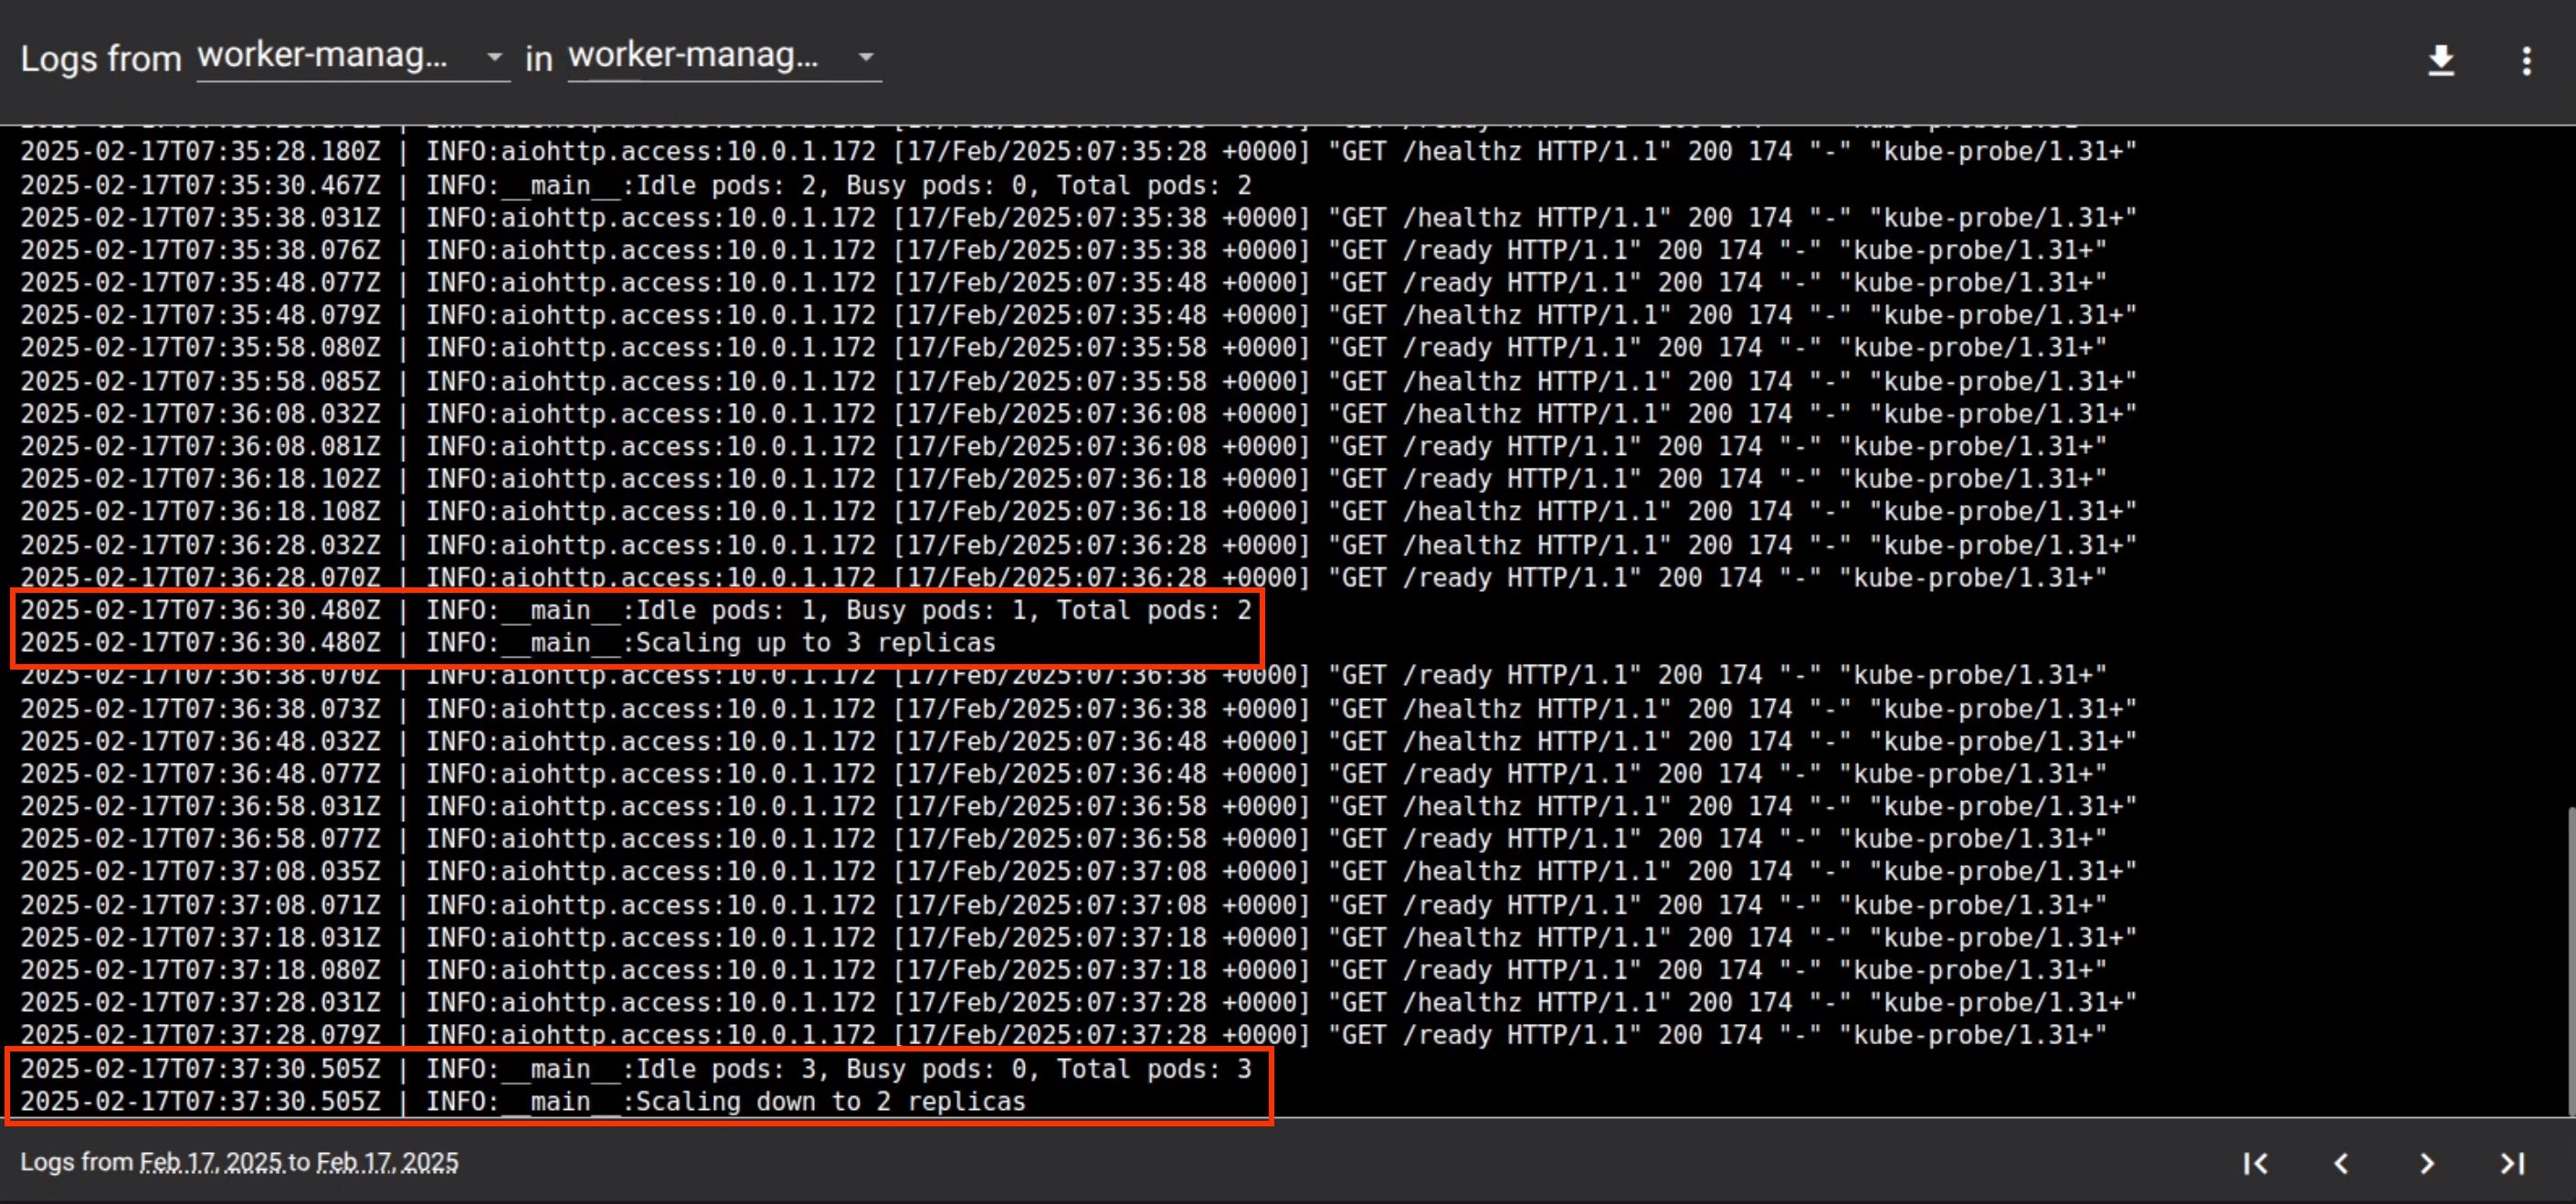
\includegraphics[width=\textwidth]{figures/worker_scaling_up_down.png}
  \caption{Worker Scaling Up and Down}
  \label{fig:worker_scaling_up_down}
\end{figure}

\subsubsection{Health and Readiness Checks}
The Worker Manager Monitor performs health and readiness checks to ensure it is ready to handle requests. These checks are essential for maintaining the reliability and availability of the system. 

Code \ref{lst:health_check} shows the implementation of the health and readiness checks.

\begin{lstlisting}[language=python, caption={Worker Manager Monitor Health and Readiness Checks}, label={lst:health_check}]
async def healthz(request):
    return web.Response(text="OK")

async def ready(request):
    # Check Redis connection
    try:
        redis_client = WorkerManagerRedisClient().get_client()
        redis_client.ping()
    except Exception as e:
        logger.error(f"Readiness check failed: Redis connection error: {str(e)}")
        return web.Response(status=500, text="Redis connection error")

    # Check if the monitor can acquire a lock
    lock_key = "readiness_check_lock"
    if not monitor.acquire_lock(lock_key, timeout=5):
        logger.error("Readiness check failed: Unable to acquire lock")
        return web.Response(status=500, text="Unable to acquire lock")
    monitor.release_lock(lock_key)

    return web.Response(text="OK")
\end{lstlisting}

The health check (\texttt{healthz}) provides a basic indicator of whether the Worker Manager Monitor is running. It responds with an "OK" message to confirm the service is active.
The readiness check (\texttt{ready}) performs the following validations to ensure the monitor is ready to function:
\begin{enumerate}
    \item \textbf{Redis Connection:} Verifies the monitor can connect to Redis by sending a \texttt{PING} request.
    \item \textbf{Lock Acquisition:} Ensures the monitor can acquire and release a distributed lock, which is critical for managing shared resources.
\end{enumerate}

When deployed on Kubernetes, it continuously monitors the readiness and liveness endpoints to determine if the service is ready to receive traffic or if it needs to be restarted. Figure \ref{fig:k8s_healthcheck} shows the successful readiness and liveness check at every 10 seconds interval.

\begin{figure}[H]
  \centering
  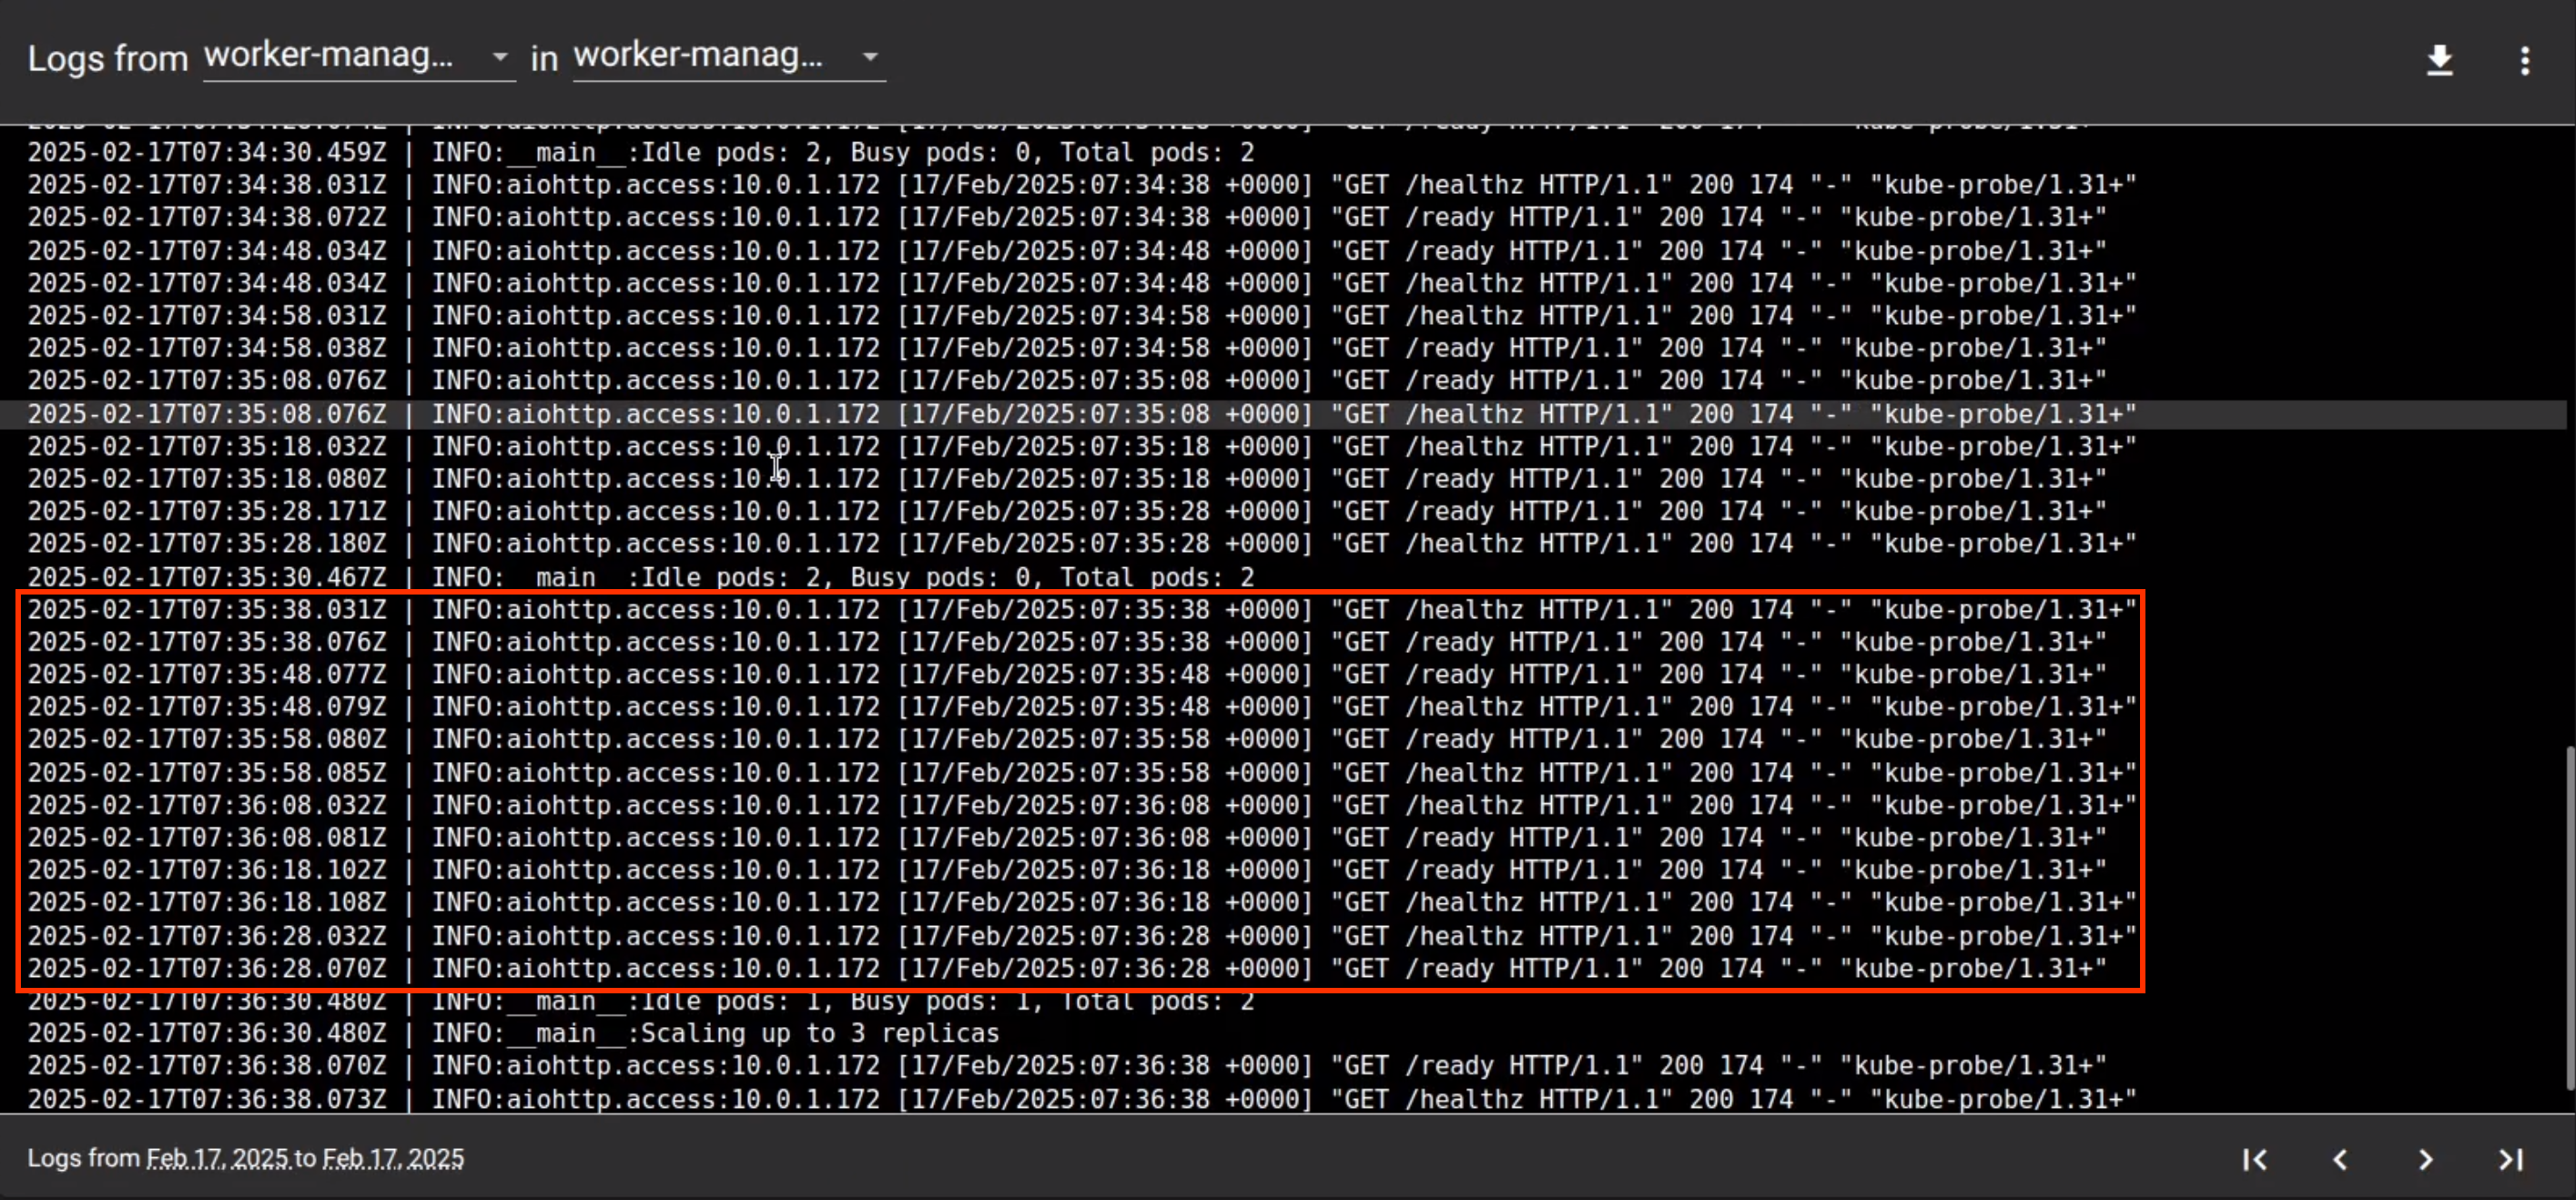
\includegraphics[width=\textwidth]{figures/k8s_healthcheck.png}
  \caption{Kubernetes Readiness and Liveness Checks}
  \label{fig:k8s_healthcheck}
\end{figure}

\section{Infrastructure Deployment}
The infrastructure is deployed using Terraform, an Infrastructure-as-Code (IaC) tool that allows for the provisioning of cloud resources in a declarative manner. Terraform compares the desired state defined in configuration files with the current state of the cloud environment and makes the necessary changes to achieve the desired state.

\subsection{AWS Access Key and CLI Configuration}
To interact with AWS services, it is necessary to create an AWS access key. This can be done by navigating to the account credentials section in the AWS Management Console and creating an access key.

Once the access key is generated, the AWS CLI can be configured by running the command:
\begin{verbatim}
  aws configure
\end{verbatim}
The CLI will prompt for the access key, secret key, region, and output format. For ease of use, a named profile can also be set up using:
\begin{verbatim}
  aws configure --profile <profile-name>
\end{verbatim}
This enables switching between different AWS accounts and regions as needed.

\subsection{Setting Up Terraform Configuration}
Terraform is used to manage infrastructure as code. There are three main Terraform commands:
\begin{itemize}
    \item \texttt{terraform init}: Initializes the configuration, downloads necessary providers, and sets up modules.
    \item \texttt{terraform plan}: Generates an execution plan to show the changes Terraform will make to the infrastructure. Code \ref{lst:terraform_plan} shows an example of the Terraform execution plan output.
    \item \texttt{terraform apply}: Applies the changes to create or update infrastructure resources. This will update our cloud environment to match the desired state defined in the Terraform configuration files.
\end{itemize}

\subsection{Storing State Files in S3}
To enable collaboration among multiple developers, the Terraform state file can be stored in an Amazon S3 bucket. The state file contains the current infrastructure state and helps Terraform determine necessary changes for future deployments.


Code \ref{lst:state_bucket} shows the Terraform configuration for setting up the state bucket. We can set the bucket name and tags as variables to customize the bucket's name and attributes. This can be done by defining the variables in a separate \texttt{variables.tf} file.

\begin{lstlisting}[language=Terraform, caption={Terraform Configuration for Setting Up State Bucket}, label={lst:state_bucket}]
resource "aws_s3_bucket" "terraform_state" {
  bucket = var.bucket_name

  tags = var.tags
}

resource "aws_s3_bucket_versioning" "terraform_state" {
  bucket = aws_s3_bucket.terraform_state.id
  versioning_configuration {
    status = "Enabled"
  }
}

resource "aws_s3_bucket_public_access_block" "terraform_state" {
  bucket = aws_s3_bucket.terraform_state.id

  block_public_acls       = true
  block_public_policy     = true
  ignore_public_acls      = true
  restrict_public_buckets = true
}
\end{lstlisting}

Amazon S3 is a highly durable, scalable, and secure object storage service provided by AWS \cite{s3}. By leveraging S3 for Terraform state file storage, teams can ensure that the state file is reliably stored and accessible across all environments. This approach also promotes collaboration, consistency, and secure infrastructure management.

To prevent race conditions when multiple developers modify the infrastructure simultaneously, a DynamoDB table \cite{dynamodb} is used to store the state lock. Code \ref{lst:dynamodb_table} shows the DynamoDB table configuration.

\begin{lstlisting}[language=Terraform, caption={Terraform Configuration for Setting Up DynamoDB Table}, label={lst:dynamodb_table}]
resource "aws_dynamodb_table" "terraform-lock" {
    name = "terraform-lock"
    hash_key = "LockID"
    read_capacity = 10
    write_capacity = 10
    
    attribute {
      name = "LockID"
      type = "S"
    }
    
    tags = {
      Name = "Terraform Lock Table"
    }
}
\end{lstlisting}

The Terraform backend configuration can then be updated to use the S3 bucket and DynamoDB table, as shown in Code~\ref{lst:backend_config}.

\begin{lstlisting}[language=Terraform, caption={Terraform Backend Configuration}, label={lst:backend_config}]
terraform {
    backend "s3" {
        bucket         = "terraform-state-bucket"
        key            = "terraform.tfstate"
        region         = "ap-southeast-1"
        dynamodb_table = "terraform-lock"
    }
}
\end{lstlisting}

\subsection{Deploying Terraform Resources}
The Terraform configuration files reference Song's Terraform modules \cite{song_yu}, with enhancements such as storing the Terraform state in an S3 bucket and simplifying deployment by creating an EFS CSI driver for the EFS volume. This driver allows Kubernetes pods to mount the EFS volume, enabling seamless integration.

The Terraform configuration for creating the EFS CSI driver and attaching it to the EFS volume is shown in Code \ref{lst:efs_csi_driver}. This configuration sets up the necessary IAM role, policy attachments, and the EFS CSI driver for an EKS cluster.

To deploy these resources, the following commands are executed:
\begin{itemize}
    \item \texttt{terraform init}: Initializes the Terraform configuration and downloads the necessary providers and modules.
    \item \texttt{terraform plan}: Generates an execution plan that shows the changes Terraform will make to the infrastructure.
    \item \texttt{terraform apply}: Applies the changes to the infrastructure and deploys the resources.
\end{itemize}

\subsection{Deploying EFS and Attaching to Models}
To store the ASR models, an Elastic File System (EFS) can be deployed. The following steps outline the deployment process:
\begin{enumerate}
    \item Create an EC2 instance in a public subnet.
    \item Attach the EFS volume to the instance.
    \item Copy the ASR model files to the EFS volume.
\end{enumerate}


Code \ref{lst:ec2_setup} shows the Terraform configuration for setting up an EC2 instance and an SSH key. 

After the EC2 instance is created, follow these steps to transfer the model files:

\begin{enumerate}
    \item Retrieve the EC2 public IP from the AWS console.
    \item SSH into the EC2 instance using \texttt{ssh -i <key.pem> ec2-user@<public-ip>}.
\end{enumerate}

On the EC2 instance:
\begin{enumerate}
    \item \texttt{sudo mkdir -p /mnt/efs}: Create a directory to mount the EFS volume.
    \item 
        \begin{sloppypar}
        \texttt{sudo mount -t nfs4 -o nfsvers=4.1 <mount-target address>:/ /mnt/efs}: Mount the EFS volume to the directory.
        \end{sloppypar}
    \item \texttt{sudo chmod go+rw /mnt/efs}: Update the permissions of the directory to allow read and write access.

    \item 
        \begin{sloppypar}
        \texttt{scp -r -i "<private key name>.pem"   \\<model-directory>@<public-ip>:/mnt/efs}: Copy the model files to the EFS volume.
        \end{sloppypar}
\end{enumerate}

\section{Kubernetes Cluster}
\texttt{kubectl} is the primary command-line tool for interacting with Kubernetes clusters. It allows users to create, update, and manage resources within the cluster. Below are some commonly used \texttt{kubectl} commands:

\begin{itemize}
    \item \texttt{kubectl apply -f <file>}: Applies the configuration defined in the YAML file to the cluster.
    \item \texttt{kubectl get <resource>}: Retrieves information about the specified resource.
    \item \texttt{kubectl describe <resource> <name>}: Provides detailed information about the specified resource.
    \item \texttt{kubectl logs <pod-name>}: Displays the logs of the specified pod.
    \item \texttt{kubectl exec -it <pod-name> -- /bin/bash}: Opens a shell in the specified pod.
    \item \texttt{kubectl delete <resource> <name>}: Deletes the specified resource.
\end{itemize}

To connect to the EKS cluster, the AWS CLI can be used to update the \texttt{kubeconfig} file with the cluster details. The following command retrieves the cluster configuration and updates the kubeconfig file:
\begin{verbatim}
aws eks --region <region> update-kubeconfig --name <cluster-name>
\end{verbatim}

Once the kubeconfig file is updated, kubectl can be used to interact with the EKS cluster.

\subsection{Deploying ASR System Components}
The ASR system can be deployed to the Kubernetes cluster using the Kubernetes manifest files provided in the repository. The deployment process can be initiated with the following command:
\begin{verbatim}
kubectl apply -f <file>
\end{verbatim}

The deployment includes the following components:
\begin{itemize}
    \item \textbf{Live Processing Service Deployment:} Deploys the Live Processing Service to manage transcription tasks.
    \item \textbf{Worker Manager Server and Monitor Deployment:} Deploys the Worker Manager Server to handle gRPC requests and the Worker Manager Monitor to manage worker health.
    \item \textbf{Worker Deployment:} Deploys the worker pods responsible for processing audio data.
    \item \textbf{Persistent Volume and Persistent Volume Claim:}  Defines the storage requirements for the EFS  volume used by the ASR system.
\end{itemize}

\subsection{Horizontal Pod Autoscaler (HPA)}
The Kubernetes Horizontal Pod Autoscaler (HPA) automatically adjusts the number of pods in a deployment based on resource utilization, such as CPU or memory, or custom metrics. This ensures efficient resource allocation and improved system responsiveness under varying workloads.

The HPA configuration is defined in a YAML file and applied to the cluster using:
\begin{verbatim}
  kubectl apply -f <file>
\end{verbatim}

Code \ref{lst:HPA_live_processing_server} provides an example HPA configuration for the Live Processing Server.


\begin{lstlisting}[language=Kubernetes, caption={Horizontal Pod Autoscaler for Live Processing Server}, label={lst:HPA_live_processing_server}]
apiVersion: autoscaling/v2
kind: HorizontalPodAutoscaler
metadata:
  name: live-processing-server-hpa
  namespace: asr-sdk
spec:
  scaleTargetRef:
    apiVersion: apps/v1
    kind: Deployment
    name: live-processing-server-deployment
  minReplicas: 2
  maxReplicas: 10
  metrics:
    - type: Resource
      resource:
        name: cpu
        target:
          type: Utilization
          averageUtilization: 75
    - type: Resource
      resource:
        name: memory
        target:
          type: Utilization
          averageUtilization: 75
\end{lstlisting}

This configuration defines the following:
\begin{itemize}
    \item \textbf{Target Deployment:} The HPA scales the \texttt{live-processing-server-deployment}.
    \item \textbf{Replica Scaling Range:} The deployment is maintained between a minimum of 2 and a maximum of 10 replicas.
    \item \textbf{Scaling Metrics:} The autoscaler monitors CPU and memory utilization, scaling up or down when usage exceeds or falls below 75\%.
\end{itemize}
\subsubsection{Testing the HPA}
To verify the HPA's behavior under load, a benchmarking tool such as \texttt{wrk} can be used to simulate traffic.

The following command generates a load test by sending 25 concurrent WebSocket requests for 30 seconds using 12 threads:
\begin{verbatim}
  wrk -t12 -c25 -d30s ws://<live-processing-service-url>/client/ws/speech
\end{verbatim}

To monitor the HPA scaling behavior in real-time, use:
\begin{verbatim}
  kubectl get hpa -n asr-sdk live-processing-server-hpa --watch
\end{verbatim}

As shown in Figure \ref{fig:hpa_cli}, after 30 seconds of sustained load, the CPU utilization surpasses the 75\% threshold, triggering the HPA to scale the deployment from 2 to 7 replicas.

\begin{figure}[!h]
  \centering
  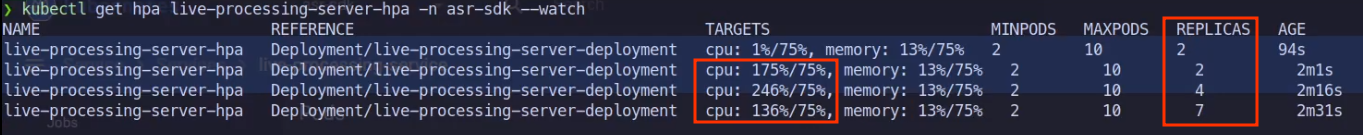
\includegraphics[width=\textwidth]{figures/hpa_cli.png}
  \caption{Testing of HPA with wrk}
  \label{fig:hpa_cli}
\end{figure}

\subsection{Helm Charts}
Helm charts were used to deploy the RabbitMQ and Redis clusters. The charts used were from Bitnami, which provides pre-configured Helm charts for popular applications, including RabbitMQ and Redis.

Users can customize their deployments by specifying configuration parameters in a \texttt{values.yaml} file. This file allows for modifications such as the number of replicas, resource limits, and persistence settings. The full list of configurable values is available in the official Helm chart repository.


The following commands deploy the Redis and RabbitMQ clusters using Helm:
\begin{verbatim}
  # Deploy Redis cluster
  helm install redis oci://registry-1.docker.io/bitnamicharts/redis \
    -f values.yaml --namespace asr-sdk --create-namespace
  
  # Deploy RabbitMQ cluster
  helm install rabbitmq oci://registry-1.docker.io/bitnamicharts/rabbitmq \
    -f values.yaml --namespace asr-sdk --create-namespace
\end{verbatim}

To ensure data persistence for RabbitMQ and Redis, Amazon Elastic Block Store (EBS) can be configured as the persistent storage backend.
\begin{enumerate}
  \item Install the EBS CSI driver on the EKS cluster if it is not already installed.
  \item Annotate the EBS CSI service account with the IAM role created for EBS via Terraform using the following command:
  \begin{verbatim} 
  kubectl annotate serviceaccount ebs-csi-controller-sa -n kube-system \
    eks.amazonaws.com/role-arn=<ARN_of_EBS_CSI_Driver_Role>
  \end{verbatim}
\end{enumerate}

\subsection{Kubernetes Dashboard}
To effectively visualize the Kubernetes cluster and monitor deployed resources, the Kubernetes Dashboard provides a graphical interface for managing the cluster, inspecting workloads, and troubleshooting issues. The dashboard allows users to view real-time metrics, manage deployments, and analyze resource utilization. Figure \ref{fig:kubernetes_dashboard} illustrates an example of the Kubernetes Dashboard.
\begin{figure}[ht]
  \centering
  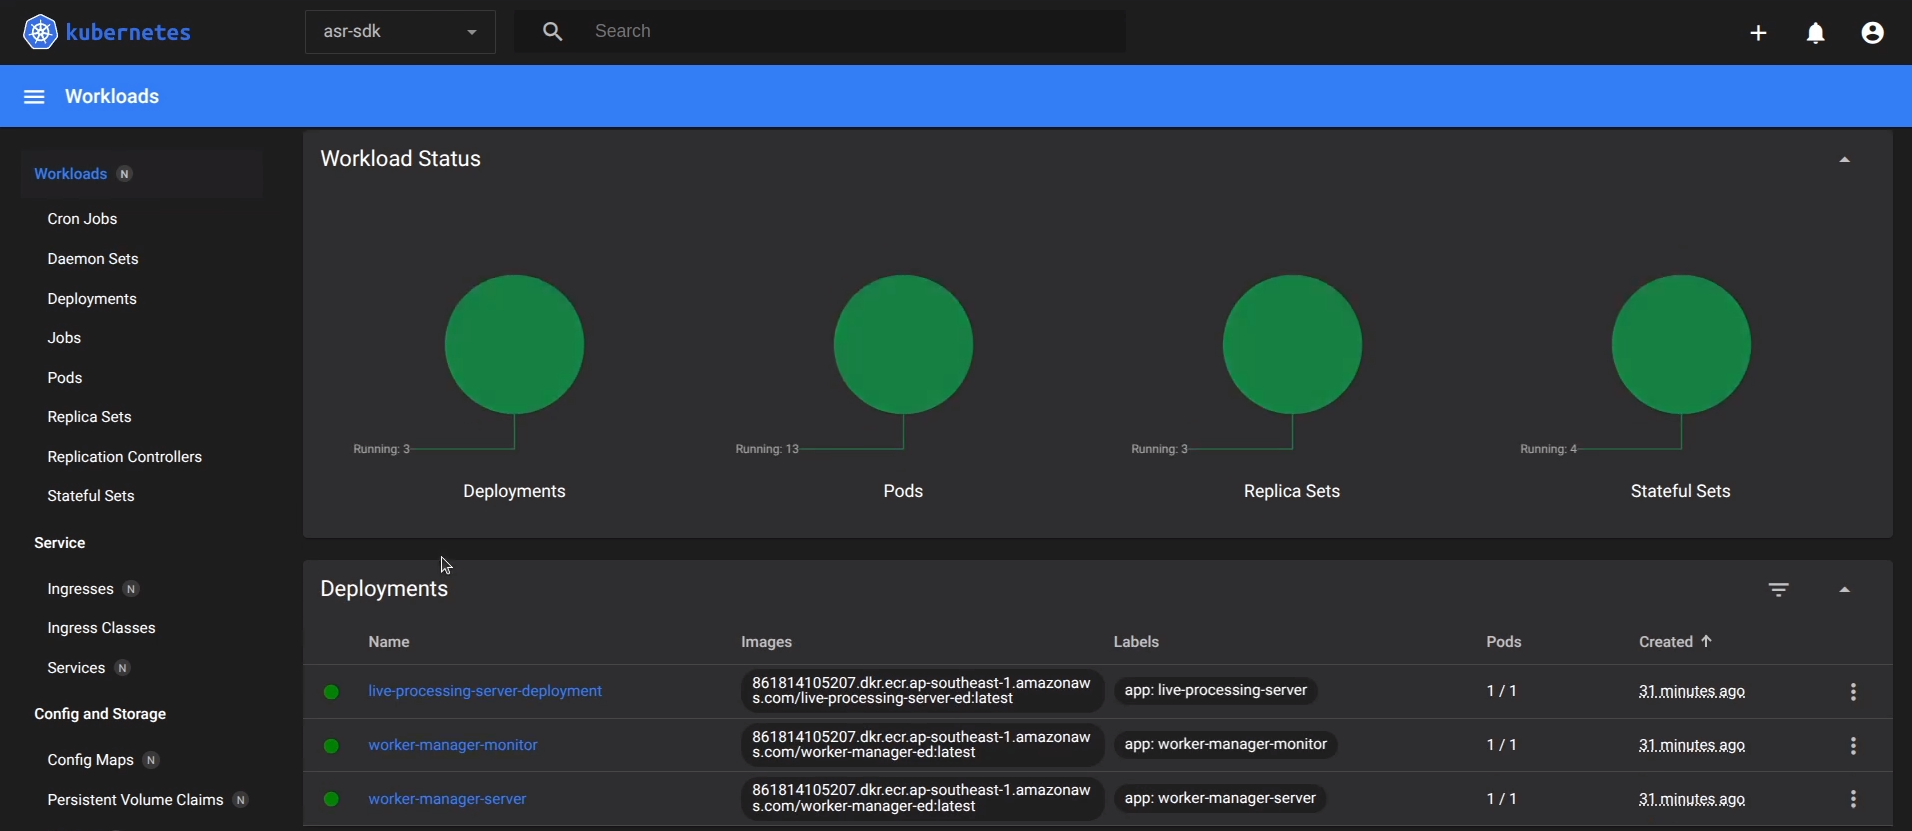
\includegraphics[width=\textwidth]{figures/kubernetes_dashboard.png}
  \caption{Kubernetes Dashboard}
  \label{fig:kubernetes_dashboard}
\end{figure}

\subsubsection{Installing the Kubernetes Dashboard}
The Kubernetes Dashboard can be installed using Helm with the following commands:

\begin{verbatim}
  helm repo add kubernetes-dashboard https://kubernetes.github.io/dashboard/
  helm upgrade --install kubernetes-dashboard \
    kubernetes-dashboard/kubernetes-dashboard \
    --create-namespace --namespace kubernetes-dashboard
\end{verbatim}

\subsubsection{Configuring Access and Permissions}
Before accessing the dashboard, a set of required resources must be configured, including:

\begin{itemize}
  \item \textbf{Service Account:} Grants access to the dashboard.
  \item \textbf{Cluster Role Binding:} Assigns permissions to the service account.
  \item \textbf{Secret Token:} Authenticates the dashboard.
\end{itemize}

The Kubernetes configuration file in Code \ref{lst:k8s_dashboard_dependencies} sets up these dependencies.


\subsubsection{Accessing the Dashboard}
Once the dashboard and necessary permissions are set up, port forwarding can be used to expose the dashboard locally:
\begin{verbatim}
  kubectl -n kubernetes-dashboard port-forward \
    svc/kubernetes-dashboard-kong-proxy 8443:443
\end{verbatim}

After running this command, open a web browser and navigate to: \texttt{https://localhost:8443}.

\subsubsection{Generating Token}
To log in to the dashboard, generate an authentication token using:
\begin{verbatim}
  kubectl -n kubernetes-dashboard create token admin-user
\end{verbatim}

\chapter{Conclusion and Future Work} \label{chapter:conclusion_and_future_work}

\textit{To be done.}



\printbibliography

\begin{appendices}
\chapter{Relevant Code Snippets} \label{chapter:appendix}

\begin{lstlisting}[caption={Example Code Documentation}, label={lst:code_documentation}]
def _start_task(self, task_queue, instance_id=1):
    """
    Start the task and set the state of the worker to BUSY.

    Args:
        task_queue (str): Task queue to be processed by the worker.
        instance_id (int): Instance ID of the task.
    """
\end{lstlisting}

\begin{lstlisting}[language=Proto3, caption={Worker Manager Server gRPC Proto File}, label={lst:worker_manager_server}]
syntax = "proto3";

package worker_manager;

service WorkerManagerService {
    rpc AllocateWorker (AllocateWorkerRequest) returns (AllocateWorkerResponse);
    rpc SendHeartbeat (SendHeartbeatRequest) returns (SendHeartbeatResponse);
}

message AllocateWorkerRequest {
    string model_name = 1;
    string task_queue = 2;
}

message AllocateWorkerResponse {
    bool success = 1;
    string worker_name = 2;
    string message = 3;
}

message SendHeartbeatRequest {
    string worker_name = 1;
    string model_name = 2;
    bool final = 3;
}

message SendHeartbeatResponse {
    bool success = 1;
    string message = 2;
}
\end{lstlisting}

\begin{lstlisting}[language=Terraform, caption={Terraform Plan Output}, label={lst:terraform_plan}]
Terraform used the selected providers to generate the following execution plan. Resource actions are indicated with the following symbols:
+ create
<= read (data resources)

Terraform will perform the following actions:

    # module.eks.aws_eks_addon.efs_csi_driver will be created
    + resource "aws_eks_addon" "efs_csi_driver" {
        + addon_name           = "aws-efs-csi-driver"
        + addon_version        = "v2.1.3-eksbuild.1"
        + arn                  = (known after apply)
        + cluster_name         = "ed-fyp-eks-cluster"
        + configuration_values = (known after apply)
        + created_at           = (known after apply)
        + id                   = (known after apply)
        + modified_at          = (known after apply)
        + tags_all             = {
            + "Environment" = "Development"
            + "Owner"       = "Edmund"
            + "Terraform"   = "True"
        }
    
... (output truncated) ...

Plan: 37 to add, 0 to change, 0 to destroy.
    
\end{lstlisting}

\begin{lstlisting}[language=Terraform, caption={Terraform Configuration for Creating EFS CSI Driver}, label={lst:efs_csi_driver},breaklines=true]
module "eks" {
    source  = "terraform-aws-modules/eks/aws"
    version = "~> 20.31"

    cluster_name    = var.cluster_name
    cluster_version = "1.31"

    vpc_id     = var.vpc_id
    subnet_ids = var.subnet_ids

    cluster_endpoint_private_access          = true
    cluster_endpoint_public_access           = true
    enable_cluster_creator_admin_permissions = true

    cluster_compute_config = {
    enabled    = true
    node_pools = ["general-purpose"]
    }
}

resource "aws_eks_addon" "efs_csi_driver" {
    cluster_name  = module.eks.cluster_name
    addon_name    = "aws-efs-csi-driver"
    addon_version = "v2.1.3-eksbuild.1"
}

resource "aws_iam_role" "efs_csi_role" {
    name = "EKS_EFS_CSI_DriverRole"
    assume_role_policy = jsonencode({
    Version = "2012-10-17"
    Statement = [
        {
        Action = [
            "sts:AssumeRoleWithWebIdentity",
        ]
        Principal = {
            Federated = "arn:aws:iam::${data.aws_caller_identity.current.account_id}: oidc-provider/${module.eks.cluster_oidc_issuer_url}"
        }
        Effect = "Allow"
        Condition = {
            StringLike = {
            "${module.eks.cluster_oidc_issuer_url}:sub" = "system:serviceaccount:kube-system:efs-csi-*",
            "${module.eks.cluster_oidc_issuer_url}:aud" = "sts.amazonaws.com"
            }
        }
        },
    ]
    })
}

resource "aws_iam_role_policy_attachment" "efs_csi_driver_policy_attachment" {
    role       = aws_iam_role.efs_csi_role.name
    policy_arn = "arn:aws:iam::aws:policy/service-role/AmazonEFSCSIDriverPolicy"
}

data "aws_caller_identity" "current" {}
\end{lstlisting}

\begin{lstlisting}[caption={Terraform Configuration for Setting Up EC2 Instance}, label={lst:ec2_setup}]
# Generate new private key
resource "tls_private_key" "my_key" {
    algorithm = "RSA"
}

# Generate a key-pair with above key
resource "aws_key_pair" "key-pair" {
    key_name   = "${var.owner}-key"
    public_key = tls_private_key.my_key.public_key_openssh
}

# Saving Key Pair for ssh login for Client if needed
resource "null_resource" "save_key_pair" {
    provisioner "local-exec" {
    command = "echo  '${tls_private_key.my_key.private_key_pem}' > '${aws_key_pair.key-pair.key_name}'.pem && chmod 400 '${aws_key_pair.key-pair.key_name}'.pem"
    }
}

# create ec2 resource for mounting model
resource "aws_instance" "ec2-instance" {
    ami                         = "ami-0e48a8a6b7dc1d30b"
    instance_type               = "t2.micro"
    key_name                    = aws_key_pair.key-pair.key_name
    subnet_id                   = var.public_subnet_ids[0]
    vpc_security_group_ids      = [var.security_group_nfs_ssh]
    associate_public_ip_address = true

    tags = {
    Name = "${var.owner}-model-transfer"
    }
}
\end{lstlisting}

\begin{lstlisting}[language=Kubernetes, caption={Kubernetes Configuration for Setting Up Dashboard Dependencies}, label={lst:k8s_dashboard_dependencies}]
apiVersion: v1
kind: ServiceAccount
metadata:
    name: admin-user
    namespace: kubernetes-dashboard
---
apiVersion: rbac.authorization.k8s.io/v1
kind: ClusterRoleBinding
metadata:
    name: admin-user
roleRef:
    apiGroup: rbac.authorization.k8s.io
    kind: ClusterRole
    name: cluster-admin
subjects:
    - kind: ServiceAccount
    name: admin-user
    namespace: kubernetes-dashboard
---
apiVersion: v1
kind: Secret
metadata:
    name: admin-user
    namespace: kubernetes-dashboard
    annotations:
    kubernetes.io/service-account.name: "admin-user"
type: kubernetes.io/service-account-token
\end{lstlisting}

\end{appendices}


\end{document}
